\documentclass[11pt]{article}
\usepackage[letterpaper,margin=1.1in]{geometry}
\usepackage{amsmath,amsthm,mathtools,booktabs,graphicx}
\usepackage{unicode-math}
\usepackage[default]{sourceserifpro}
\usepackage[scale=0.92]{plex-sans}
\setmathfont{LibertinusMath-Regular.otf}
\usepackage[authoryear,round]{natbib}
\usepackage{xcolor}
\definecolor{accent}{HTML}{27548A}
\definecolor{muted}{HTML}{5F6B7A}
\usepackage[font={small},labelfont={sf,bf},labelsep=period]{caption}
\usepackage{titlesec}
\titleformat*{\section}{\sffamily\large\bfseries}
\titleformat*{\subsection}{\sffamily\normalsize\bfseries}
\titleformat{\paragraph}[runin]{\sffamily\small\bfseries}{}{}{}[.]
\titlespacing*{\paragraph}{0pt}{1.2ex plus .4ex}{.6em}
\usepackage{enumitem}
\setlist{itemsep=2pt,topsep=4pt}
\usepackage[colorlinks=true,linkcolor=accent,citecolor=accent,urlcolor=accent]{hyperref}
\hypersetup{pdftitle={The topology of range-measurement credible regions},pdfauthor={Meet Mehta},
  pdfsubject={Mathematical statistics},
  pdfkeywords={highest-posterior-density region, Betti number, Morse theory, range measurement, flip ambiguity}}
\graphicspath{{figs/}}
\linespread{1.06}
\frenchspacing

\newtheoremstyle{sfplain}{1.1ex}{1.1ex}{\normalfont}{}{\sffamily\bfseries}{.}{.5em}{}
\newtheoremstyle{sfremark}{1.1ex}{1.1ex}{\normalfont}{}{\sffamily\itshape}{.}{.5em}{}
\theoremstyle{sfplain}
\newtheorem{theorem}{Theorem}[section]
\newtheorem{lemma}[theorem]{Lemma}
\newtheorem{proposition}[theorem]{Proposition}
\newtheorem{corollary}[theorem]{Corollary}
\theoremstyle{sfremark}
\newtheorem{remark}[theorem]{Remark}
\newtheorem{conjecture}[theorem]{Conjecture}
\renewcommand{\qedsymbol}{\textcolor{muted}{\openbox}}

\newcommand{\R}{\mathbb{R}}
\newcommand{\HPD}{\mathcal{H}_\alpha}
\newcommand{\dd}{\,\mathrm{d}}
\DeclareMathOperator{\Cov}{Cov}
\DeclareMathOperator{\tr}{tr}

\title{\sffamily\bfseries The topology of range-measurement credible regions}
\author{Meet Mehta\\[2pt] \small\texttt{meetmehta.5410@gmail.com}}
\date{}

\begin{document}
\maketitle

\begin{abstract}\noindent
Noisy distances from a point to known anchors give posteriors whose credible regions are rings, shells, tubes and
disconnected pieces rather than ellipses. We determine their topology exactly. The key observation is that for two ranges,
in residual coordinates (the differences between distances and observed ranges), the posterior is a Gaussian times an
explicit weight on a convex polygonal domain, and every highest-posterior-density region is a disc cut by the walls
of that domain. Its topology can therefore be read off the triangle whose sides are the anchor separation and the two
observed ranges. This gives the complete sequence of topologies as the noise grows, in every dimension: each transition
occurs when the cut-off reaches one of five depths, the squared incircle tangent lengths $t_*^2, t_1^2, t_2^2$ and the
sums $t_*^2 + t_1^2$, $t_*^2 + t_2^2$, and more noise first creates holes and then removes them. With a different noise
level on each range the disc becomes an ellipse, and a contact can annihilate with an anchor. For $n \le d$ ranges the
noise-free shape persists while the region misses the affine hull of the anchors, and for $n = d$ only then. An explicit
noise level, computable from the data, certifies the noise-free shape. In simulation, from the noise level at which the first hole forms, even a mixture of
Laplace approximations at the two posterior modes covers the true point in only 84--93\% of data sets at the 95\% level. For one range the region has a hole exactly
when $r/\sigma$ exceeds $\kappa_d = \sqrt{d/2} + z\sqrt{3/8} + O(d^{-1/2})$, and the posterior mean then lies in the hole.
In high dimension every transition has an explicit limit with a $1/\sqrt d$ correction, and for random anchors in the
plane the flip pair is lost with probability of order $\sqrt\sigma$, up to a logarithmic factor.

\end{abstract}

\noindent{\sffamily\small\textbf{Keywords:} highest-posterior-density region, Betti number, Morse theory, range
measurement, flip ambiguity, Laplace method.}\\[2pt]
{\sffamily\small\textbf{MSC 2020:} Primary 62F15; secondary 55N31, 57R70, 62E20, 60D05.}

%======================================================================
\section{Introduction}

Measure the distance from an unknown point to a known anchor, with noise. The data cannot tell direction, so the
posterior spreads around a sphere centred at the anchor, and its 95\% credible region is a ring in the plane or a
spherical shell in space. A second range cuts the sphere down to the intersection of two spheres: two points in the
plane, a circle in space. Each measurement changes the shape of what is known, not only its size
(Figure~\ref{fig:staircase}). When the noise grows the shapes thicken, merge and fill in, and the credible region passes
through a sequence of topologies before it becomes a ball.

These shapes are where standard summaries fail. Localisation from distances, in GNSS ranging, sonar, ultra-wideband and
wireless sensor networks \citep{gustafsson2005,patwari2005,mao2007}, routinely reports a point estimate with a covariance
ellipse \citep{kay1993}, or approximates the posterior by a Gaussian through a Laplace approximation \citep{tierney1986}
or an extended Kalman filter \citep{jazwinski1970}. Every such summary has a convex credible region. Particle methods and
nonparametric belief propagation can carry multimodal posteriors \citep{doucet2001,thrun2005,ihler2005}, but their output
is still read through means, covariances or modes. The Bernstein--von Mises theorem \citep[Chapter~10]{vandervaart1998}
explains why Gaussian summaries usually work as data accumulate, and the Laplace method does the same here, with one
observation per anchor and small noise; both need the posterior to concentrate at an isolated, non-degenerate mode. With $n \le d$ ranges in $\R^d$ there is none: generically the noise-free solutions form a $(d - n)$-sphere, a
mirror pair when $n = d$. When the true region is a shell, or two separate pieces, a Gaussian summary is wrong in kind
and its centre may lie where the data rule the target out. The question we answer is exact: for which noise levels does
the credible region have which topology?

\begin{figure}[t]\centering
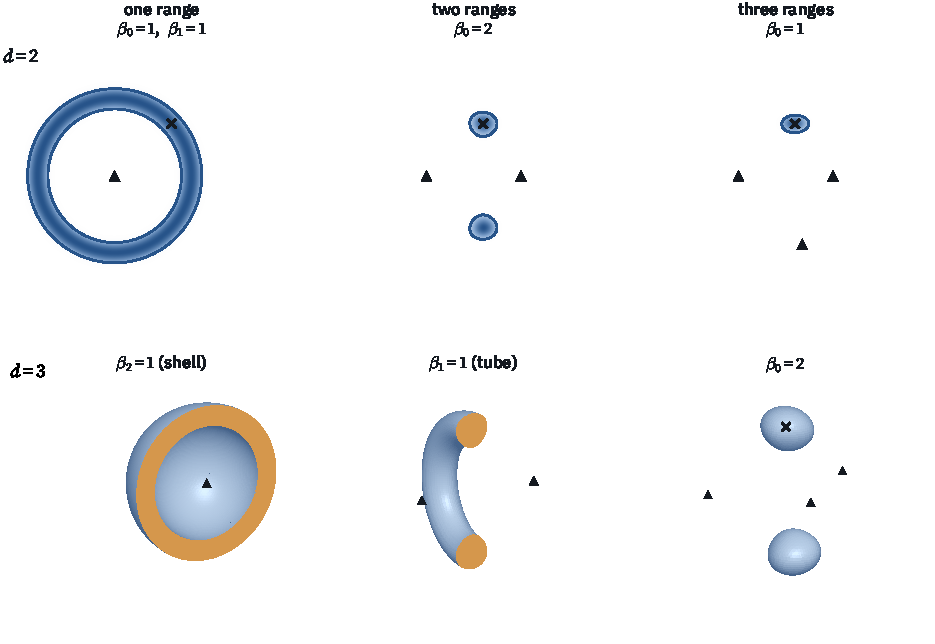
\includegraphics[width=\linewidth]{fig1_staircase.pdf}
\caption{Highest-posterior-density (HPD) regions at 95\% as ranges are added, in the plane (top) and in space (bottom),
at small noise. One range gives a ring or a shell, two give two pieces (the flip ambiguity) or a tube, three give one piece
in the plane and two in space. Triangles mark the anchors and a cross the true point. In the plane, colour is posterior
density inside the region; in space, the shell and the tube are cut open along a plane through the anchors, and the
cut face is amber. Every panel's Betti numbers were confirmed by direct computation.}
\label{fig:staircase}
\end{figure}

\paragraph{Results}
\begin{itemize}[leftmargin=1.2em]
\item \emph{Monotone depth} (Theorem~\ref{thm:depth}). For any number of ranges, the HPD region is a sublevel set
$\{\Delta \le \Delta_\alpha(\sigma)\}$ of the depth $\Delta = (S - \min S)/2$, and $\Delta_\alpha(\sigma)$ increases
strictly with the noise, so it crosses each critical depth of $S$ exactly once, in increasing order, in every
dimension.
\item \emph{One range} (Theorem~\ref{thm:main}). The region has a hole if and only if $r/\sigma > \kappa_d(\alpha)$;
$\kappa_d$ increases with $d$ and has the three-term expansion of Theorem~\ref{thm:main}(c), with $\kappa_2 = 1.996$ at 95\%. The threshold exists for every
noise whose negative log-density is convex in $\log|\varepsilon|$ (Theorem~\ref{thm:noise}); its growth law does not, and for
Laplace noise the threshold grows like $d/2 + (z/2)\sqrt d$ (Proposition~\ref{prop:laplace}). The posterior mean lies in the
hole, and the moment-matched Gaussian has none (Corollary~\ref{cor:mean}, Proposition~\ref{prop:gauss}).
\item \emph{Two ranges} (Theorem~\ref{thm:triangle}, Proposition~\ref{prop:axis}). Residual coordinates turn the
posterior into a Gaussian times an explicit weight on a half-strip whose walls lie at distances
$\sqrt2\,t_*, \sqrt2\,t_1, \sqrt2\,t_2$ from the origin: the incircle tangent lengths, scaled by $\sqrt 2$, of the
triangle with sides the anchor separation and the two observed ranges. Every transition
is the disc of the HPD region touching a wall or swallowing a corner (Figure~\ref{fig:residual}), and the full sequence
of topologies follows in every dimension.
\item \emph{Unequal noise} (Theorem~\ref{thm:unequal}). With a different noise level on each range the disc becomes an
ellipse. A contact and an anchor can then annihilate, so a hole that equal noise would create never forms; this happens at
most once, always at the noisier anchor, and never as the first event.
\item \emph{Three ranges in the plane} (Theorem~\ref{thm:far}, Proposition~\ref{prop:birth}). A hole can surround no
anchor: for distant truths the last hole closes at the Fermat point of the anchors, and the centre of the last hole
passes from an anchor to the Fermat point through a fold at an explicit distance.
\item \emph{Up to $d$ ranges} (Theorem~\ref{thm:nranges}). For $n \le d$ affinely independent anchors the region has
the noise-free shape, a thickened $(d - n)$-sphere, while it misses the affine hull of the anchors; for $n = d$ it is
two pieces exactly then.
\item \emph{A certified staircase} (Theorems~\ref{thm:staircase} and~\ref{thm:staircaseW}). An explicit $\sigma_1$, a
formula in the observed triangle, $d$, $\alpha$ and the noise ratio, below which the region provably has the noise-free
topology; it is computable from the data.
\item \emph{High dimension} (Theorem~\ref{thm:high}). The posterior concentrates at the maximiser of a strictly
concave function on the half-strip, and every transition has an explicit limit with a $1/\sqrt d$ correction: at a
right angle, $0.7286 - 1.256/\sqrt d$ in units where the ranges are $\sqrt d$.
\item \emph{Random anchors} (Theorems~\ref{thm:sqrt2} and~\ref{thm:random2}). For one range the probability of a hole
jumps from 1 to 0 at $\sigma = \sqrt 2$, with an explicit scaling limit in a window of width $1/\sqrt d$. For two ranges
the region is a tube below $0.7286$, contractible up to $\sqrt2$, has two cavities up to $1.5062$, and is contractible
beyond. In the plane, the probability that the region is not two pieces is of order $\sqrt\sigma$, up to a factor
$(\log 1/\sigma)^{1/4}$ (Theorem~\ref{thm:sqrtlaw}).
\end{itemize}

\begin{figure}[t]\centering
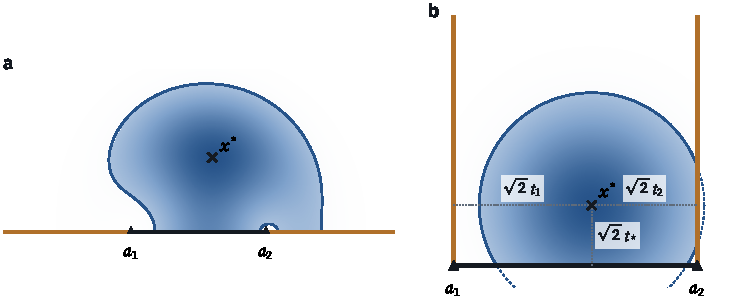
\includegraphics[width=\linewidth]{fig10_residual.pdf}
\caption{The key change of variables, for two ranges in the plane: $D = 2$, $x^* = (0.2, 1.1)$, $\sigma = 0.56$. (a) The
95\% HPD region in the upper half-plane; the anchor line consists of the segment $[a_1, a_2]$ (black) and the two outer
rays (amber). (b) The same region in the residual coordinates of Lemma~\ref{lem:residual}, rotated to $\bigl((e_1 - e_2)/\sqrt2, (e_1 + e_2)/\sqrt2\bigr)$: the half-plane becomes a half-strip whose walls are
the images of the segment and the rays, at distances $\sqrt2\,t_*$, $\sqrt2\,t_1$, $\sqrt2\,t_2$ from $x^*$, and the
region becomes the disc $|e|^2 \le 2\Delta_\alpha$ cut by the walls. Here the disc crosses the base and the wall beyond
$a_2$ but not the corner $a_2$, so the region meets the axis in two intervals ($m = 2$), and the full region, (a) together
with its mirror image, has one hole.}
\label{fig:residual}
\end{figure}

\paragraph{Related work}
\emph{Credible regions and level sets.} Highest-posterior-density regions are a standard Bayesian summary
\citep{boxtiao1973,berger1985}; \citet{hyndman1996} showed how to compute and display them and stressed that they can
be disjoint, and \citet{chenshao1999} estimate HPD intervals by Monte Carlo. An HPD region is a superlevel set of the posterior,
and density level sets have a long statistical history: as cluster definitions \citep{hartigan1975,rinaldo2010,chacon2015},
through the excess mass \citep{polonik1995}, with minimax rates \citep{tsybakov1997}, and with confidence sets and
visualisation \citep{chen2017}; inference for modes is developed by \citet{genovese2016}. That literature estimates level
sets of an unknown density from data. Here the density is known, and the question is how the topology of its level sets
is organised and when it changes. \citet[Theorem~2]{tommei2026} proves that the first two moments do not determine the number of
connected components of highest-density credible sets, using a constructed pair of smooth densities, and
\citet[Theorem~3]{tommei2026} shows that within a $C^2$ family the credible sets at fixed mass keep their isotopy type
until the threshold crosses a critical point. Our Proposition~\ref{prop:gauss} is a natural, dimension-indexed
counterpart of the first for holes at a sharp threshold, at a non-smooth point outside the hypotheses of the second.

\emph{Topology.} Topological data analysis \citep{carlsson2009,edelsbrunner2010,wasserman2018} estimates homology from
samples: \citet{bobrowski2017} recover the homology of density level sets and \citet{fasy2014} build confidence sets for
persistence diagrams. The topology of excursion sets of random fields is treated by \citet{adler2007}, and
\citet{rohrscheidt2024} use topology as a tool for Bayesian computation. We compute the topology of a posterior's
credible regions exactly, by Morse theory \citep{milnor1963}. The anchors are critical points at which the function
itself is not differentiable: near an anchor $a_i$, $S$ is a smooth function minus $2r_i\|x - a_i\|$. Stratified Morse
theory \citep{goresky1988} extends the classical theory to singular spaces rather than singular functions; critical-point
theory for distance functions \citep{groveshiohama1977,grove1993} and Morse theory for piecewise-smooth functions
\citep{agrachev1997} do allow non-smooth functions, but neither applies to this cone point as it stands, and it is simple
enough to treat directly. \citet{carreira2003} showed that
Gaussian mixtures can have more modes than components, an early instance of a density's critical-point structure
departing from its parametrisation; our setting is the simplest place where such a departure is a hole rather than an
extra mode.

\emph{Localisation.} Flip ambiguity, in which a node's position is reflected through the line of its neighbours, is the
two-range staircase. It is analysed through graph rigidity by \citet{eren2004} and \citet{aspnes2006}, avoided with robust
quadrilaterals by \citet{moore2004}, and quantified by \citet{kannan2010}, all for noise-free or worst-case
configurations. In range-only SLAM, ring-shaped and multimodal beliefs are routine and are carried by sums of Gaussians,
particle filters or filters in polar coordinates \citep{blanco2008,djugash2012}. We give the corresponding statement for
Bayesian credible regions: the exact noise levels at which the
flip pair merges, and a certified level below which it provably has not.

\paragraph{Outline} Section~\ref{sec:setting} sets up the model and proves the monotone-depth principle.
Section~\ref{sec:one} treats one range: the threshold $\kappa_d$, other noise laws, and the excluded mean.
Section~\ref{sec:two} treats two ranges through residual coordinates, with equal and unequal noise levels, and up to
$d$ ranges; Section~\ref{sec:staircase} certifies the staircase. Section~\ref{sec:high} is the high-dimensional limit,
and Section~\ref{sec:random} treats random anchors. Appendix~\ref{app:sqrt} proves the square-root law. The
Supplementary Material contains the proofs of Theorem~\ref{thm:main}(c) and of Sections~\ref{sec:three}
and~\ref{sec:high} (Supplements~\ref{app:c}--\ref{app:high}) and the computations (Supplement~\ref{app:comp}).

\paragraph{Notation} $\|\cdot\|$ is the Euclidean norm, $S^k$ the unit $k$-sphere, $\Phi$ and $\varphi$ the standard
normal distribution function and density, and $z = \Phi^{-1}(1-\alpha)$. $\beta_k(X)$ is the $k$-th Betti number, the
rank of $H_k(X;\mathbb Q)$ \citep{hatcher2002}; $\simeq$ denotes homotopy equivalence, $\cong$ homeomorphism,
$\bigvee_m$ a wedge of $m$ copies and $\Sigma$ suspension. $\Pi_\sigma$ is the posterior probability measure.

%======================================================================
\section{Setting and the monotone-depth principle}\label{sec:setting}

\paragraph{Model} Anchors $a_1, \dots, a_n \in \R^d$ are known, $x \in \R^d$ is unknown, and we observe
$r_i = \|x - a_i\| + \varepsilon_i$ with $\varepsilon_i$ independent $N(0, \sigma^2)$, $\sigma > 0$ known. With the flat
prior the posterior density is
\[ p(x) \propto e^{-S(x)/2\sigma^2}, \qquad S(x) = \sum_{i=1}^n \bigl(\|x - a_i\| - r_i\bigr)^2 . \]
It is proper: $S \ge (\|x - a_1\| - r_1)^2$ and $\int e^{-(\|x - a_1\| - r_1)^2/2\sigma^2}\dd x < \infty$ (\S\ref{sec:one}).
We call
\[ \Delta(x) = \tfrac12\bigl(S(x) - \min S\bigr) \]
the \emph{depth} of $x$, so that $p(x) = p_{\max}\,e^{-\Delta(x)/\sigma^2}$.

\paragraph{Credible regions} The $1-\alpha$ highest-posterior-density region $\HPD$ is the smallest superlevel set
of $p$ with posterior mass at least $1-\alpha$. Since $p$ is a decreasing function of $\Delta$,
$\HPD = \{\Delta \le \Delta_\alpha(\sigma)\}$, where $\Delta_\alpha(\sigma)$ is the unique $\delta$ with
$\Pi_\sigma(\Delta \le \delta) = 1-\alpha$. This $\delta$ is unique because $\delta \mapsto \Pi_\sigma(\Delta \le \delta)$ is
continuous (level sets of $S$ are null: $S$ is real-analytic and non-constant off the anchors) and strictly increasing
($\{\delta < \Delta < \delta'\}$ is open and, $S$ being continuous and unbounded, non-empty).

\paragraph{Critical depths} The \emph{depth} of a critical point $x_c$ of $S$ is $\Delta_c = \Delta(x_c)$; the anchors,
where $S$ is not differentiable, are treated directly where they occur.

\begin{theorem}[Monotone depth]\label{thm:depth}
For any anchors, ranges and dimension, $\Delta_\alpha(\sigma)$ is continuous and strictly increasing in $\sigma$, with
$\Delta_\alpha(\sigma) \to 0$ as $\sigma \to 0$ and $\Delta_\alpha(\sigma) \to \infty$ as $\sigma \to \infty$. Hence each
critical depth $\Delta_c > 0$ is reached at exactly one noise level, and these crossings occur in increasing order of
$\Delta_c$.
\end{theorem}

\begin{proof}
With $\tau = 1/\sigma^2$ the posterior is the exponential family $p_\tau \propto e^{-\tau\Delta}$. For $\tau \ge \tau_0 > 0$
the integrands $(1 + \Delta)e^{-\tau\Delta}$ are dominated by $(1 + \Delta)e^{-\tau_0\Delta}$, which is integrable, so we
may differentiate under the integral \citep[Chapter~2]{brown1986}. For a fixed $\delta$ and $A = \{\Delta \le \delta\}$,
\[ \frac{\dd}{\dd\tau}\Pi_\tau(A) = \Cov_\tau(1_A, -\Delta)
   = \Pi_\tau(A)\,\Pi_\tau(A^c)\,\bigl(E_\tau[\Delta \mid A^c] - E_\tau[\Delta \mid A]\bigr) > 0, \]
because $\Delta \le \delta$ on $A$ and $\Delta > \delta$ on $A^c$. So $\Pi_\sigma(\Delta \le \delta)$ is continuous and
strictly decreasing in $\sigma$, and strictly increasing in $\delta$; hence $\Delta_\alpha(\sigma)$ is continuous and
strictly increasing.

For the limits, let $\delta > 0$ and $U = \{\Delta < \delta/4\}$, a non-empty open set. For $\sigma \le 1$,
on $\{\Delta > \delta\}$ we have $\Delta/\sigma^2 \ge \delta/2\sigma^2 + \Delta/2$, so
\[ \Pi_\sigma(\Delta > \delta) \le \frac{e^{-\delta/2\sigma^2}\int e^{-\Delta/2}}{|U|\,e^{-\delta/4\sigma^2}}
   = C\,e^{-\delta/4\sigma^2} \to 0 , \]
and $\Delta_\alpha(\sigma) < \delta$ for small $\sigma$. As $\sigma \to \infty$, $\{\Delta \le \delta\}$ is bounded while
$\int e^{-\Delta/\sigma^2} \to \infty$ by monotone convergence, so $\Pi_\sigma(\Delta \le \delta) \to 0$.
\end{proof}

The proof is a sorting argument: every point inside the cut-off has a larger sufficient statistic $-\Delta$ than every
point outside it, so raising the precision can only move mass inward. The same sorting proves the one-range threshold
below. Away from the anchors, sublevel sets of $S$ change topology only at critical values \citep{milnor1963}, so
Theorem~\ref{thm:depth} turns the question ``at which noise level does the topology change?'' into locating the critical
points of $S$ and their depths, which depend on the geometry alone, not on $\sigma$ or $d$. Theorem~\ref{thm:depth} does
not by itself say which changes occur: critical points can be degenerate, can share a depth, or can sit at the anchors,
where $S$ is not differentiable. Sections~\ref{sec:one} and~\ref{sec:two} settle this completely for one and two ranges.

%======================================================================
\section{One range}\label{sec:one}

Let $n = 1$, with anchor $a$ and range $r > 0$, and write $w = \|x - a\|$ and $\kappa = r/\sigma$. If $r \le 0$ the
density decreases in $w$ and every HPD region is a ball; we exclude this case. Define, for $\kappa > 0$ and $q \ge 0$,
\[ M_d(\kappa) = \frac{\int_0^{2\kappa} u^{d-1} e^{-(u-\kappa)^2/2}\dd u}{\int_0^{\infty} u^{d-1} e^{-(u-\kappa)^2/2}\dd u},
   \qquad
   P_d(\kappa, q) = \frac{\int_{\max(0,\kappa-q)}^{\kappa+q} u^{d-1} e^{-(u-\kappa)^2/2}\dd u}{\int_0^{\infty} u^{d-1} e^{-(u-\kappa)^2/2}\dd u}. \]
We say that $\HPD$ \emph{has a hole} if $a \notin \HPD$.

\begin{lemma}[Shells]\label{lem:shell}
$\HPD = \{x : |w - r| \le \sigma q_\alpha\}$, where $q_\alpha$ is the unique $q \ge 0$ with $P_d(\kappa, q) = 1 - \alpha$.
$\HPD$ has a hole if and only if $M_d(\kappa) > 1 - \alpha$. In that case $\HPD$ is the closed shell
$\{x : r - \sigma q_\alpha \le w \le r + \sigma q_\alpha\}$, whose inner radius is positive, homeomorphic to $S^{d-1} \times [0,1]$, so
$\beta_{d-1}(\HPD) = 1$ for $d \ge 2$ and $\beta_0(\HPD) = 2$ for $d = 1$. Otherwise $\HPD$ is a closed ball.
\end{lemma}

\begin{proof}
Here $\Delta = (w - r)^2/2$, so superlevel sets of $p$ are the shells $\{|w - r| \le \sigma q\}$. In polar coordinates about
$a$, $\dd x = w^{d-1}\dd w\dd\vartheta$; substituting $u = w/\sigma$, the mass of the shell is $P_d(\kappa, q)$, which is
continuous and strictly increasing in $q$, from $0$ to $1$. The anchor lies in the shell if and only if
$q_\alpha \ge \kappa$, i.e.\ $P_d(\kappa,\kappa) \le 1 - \alpha$, and $P_d(\kappa,\kappa) = M_d(\kappa)$.
\end{proof}

\subsection{The threshold}

\begin{theorem}\label{thm:main}
Fix $\alpha \in (0,1)$.
\begin{enumerate}[label=(\alph*)]
\item $M_d$ is continuous and strictly increasing on $(0,\infty)$, from $0$ to $1$. Hence there is a unique
$\kappa_d(\alpha)$ with $M_d(\kappa_d(\alpha)) = 1-\alpha$, and $\HPD$ has a hole if and only if $r/\sigma > \kappa_d(\alpha)$.
\item $M_{d+1} < M_d$ on $(0, \infty)$. Hence $\kappa_{d+1}(\alpha) > \kappa_d(\alpha)$.
\item As $d \to \infty$, with the implied constant depending on $\alpha$,
\[ \kappa_d(\alpha) = \sqrt{d/2} + z\sqrt{3/8} + \frac{c_\alpha}{\sqrt d} + O(1/d), \qquad
   c_\alpha = \frac{13z^2 - 28}{72\sqrt2}. \]
At $\alpha = 0.05$: $z\sqrt{3/8} = 1.00726$ and $c_\alpha = 0.0704$.
\item $\kappa_1(\alpha) = \Phi^{-1}(1/(1+\alpha))$, and $\kappa_2(\alpha)$ is the unique root of
$\kappa(2\Phi(\kappa) - 1) = (1-\alpha)(\kappa\Phi(\kappa) + \varphi(\kappa))$. At $\alpha = 0.05$, $\kappa_1 = 1.6684$
and $\kappa_2 = 1.9962$.
\end{enumerate}
\end{theorem}

\begin{proof}[Proof of (a)]
Put $u = \kappa v$. The powers of $\kappa$ cancel and the cut-off $2\kappa$ becomes $v = 2$:
$M_d(\kappa) = \Pr_\tau(W \le 2)$, where $W$ has density $\propto v^{d-1}e^{\tau T(v)}$ on $(0,\infty)$, $\tau = \kappa^2$ and
$T(v) = -(v-1)^2/2$. This is an exponential family in $\tau$ and, as in Theorem~\ref{thm:depth},
$\frac{\dd}{\dd\tau}\Pr_\tau(A) = \Pr_\tau(A)\Pr_\tau(A^c)\bigl(E_\tau[T \mid A] - E_\tau[T \mid A^c]\bigr)$ for
$A = \{W \le 2\}$. On $A$,
$(v-1)^2 < 1$ almost surely, so $T > -1/2$; on $A^c$, $T < -1/2$. Hence $M_d$ is $C^1$ and strictly increasing. As
$\kappa \to 0$ the numerator of $M_d$ is at most $(2\kappa)^d/d$ while the denominator tends to
$\int_0^\infty u^{d-1}e^{-u^2/2}\dd u > 0$. As $\kappa \to \infty$, the numerator of $1 - M_d$ is
$\int_\kappa^\infty (v+\kappa)^{d-1}e^{-v^2/2}\dd v = O(\kappa^{d-2}e^{-\kappa^2/2})$ and the denominator is at least
$2e^{-1/2}(\kappa-1)^{d-1}$. Lemma~\ref{lem:shell} gives the hole criterion.
\end{proof}

The hole's edge $v = 2$ is exactly where $(v-1)^2$ crosses $1$, which is why the sorting works.

\begin{proof}[Proof of (b)]
Let $U_d$ have density $\propto u^{d-1}e^{-(u-\kappa)^2/2}$ on $(0, \infty)$. One more dimension multiplies the density
by $u$, so for $c > 0$
\[ \Pr(U_{d+1} \le c) = \Pr(U_d \le c)\,\frac{E[U_d \mid U_d \le c]}{E[U_d]} < \Pr(U_d \le c), \]
since $E[U_d \mid U_d \le c] < c < E[U_d \mid U_d > c]$. Take $c = 2\kappa$. Then
$M_{d+1}(\kappa_d) < 1 - \alpha = M_{d+1}(\kappa_{d+1})$, and (a) gives $\kappa_d < \kappa_{d+1}$.
\end{proof}

\begin{proof}[Proof of (d)]
Substitute $v = u - \kappa$. For $d = 1$, $M_1(\kappa) = (2\Phi(\kappa) - 1)/\Phi(\kappa)$. For $d = 2$, the odd part
$\int_{-\kappa}^{\kappa} v e^{-v^2/2}\dd v$ vanishes and $\int_{-\kappa}^\infty v e^{-v^2/2}\dd v = e^{-\kappa^2/2}$, so
$M_2(\kappa) = \kappa(2\Phi(\kappa) - 1)/(\kappa\Phi(\kappa) + \varphi(\kappa))$.
\end{proof}

Part (c) is proved in Supplement~\ref{app:c}. The idea: after centring at its mode $u^* \approx \sqrt{2d}$ the radial
variable is asymptotically Gaussian with variance $2/3$. Writing $\kappa = \sqrt{d/2} + \delta$, the hole's edge
$2\kappa$ sits $\tfrac43\delta$ above the mode, so $M_d \to \Phi(\delta\sqrt{8/3})$ and $\delta \to z\sqrt{3/8}$; the
next term is the Edgeworth correction \citep{hall1992} from the skewness of $U$, of order $1/\sqrt d$. Part (b) has a geometric reading:
the volume factor $w^{d-1}$ puts more mass outside the radius $r$ than inside it, increasingly so with $d$, so the
shell must widen to hold $1-\alpha$ and its inner edge reaches the anchor at a smaller noise level $r/\kappa_d$.

\begin{figure}[t]\centering
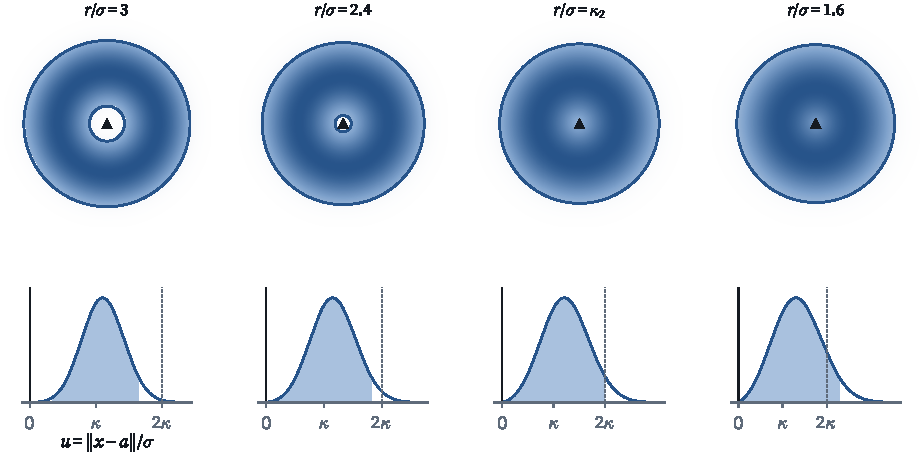
\includegraphics[width=\linewidth]{fig2_one_range.pdf}
\caption{One range in the plane, $r/\sigma = 3$, $2.4$, $\kappa_2 = 1.996$ and $1.6$. Top: the 95\% HPD region. Bottom:
the posterior density of $u = \|x - a\|/\sigma$, with the HPD interval shaded. The region has a hole exactly while the
interval excludes $0$, that is, while $[0, 2\kappa]$ holds more than 95\% of the mass (Lemma~\ref{lem:shell}); the hole
closes at $r/\sigma = \kappa_2$.}
\label{fig:onerange}
\end{figure}

\begin{table}[t]\centering\small
\caption{The threshold $\kappa_d(\alpha)$ to six decimals (Supplement~\ref{app:comp}).}\label{tab:kappa}
\begin{tabular}{rcc@{\qquad}rcc}\toprule
$d$ & $\alpha = 0.05$ & $\alpha = 0.01$ & $d$ & $\alpha = 0.05$ & $\alpha = 0.01$\\\midrule
1 & 1.668391 & 2.330079 & 6 & 2.745700 & 3.279081\\
2 & 1.996153 & 2.595899 & 7 & 2.885292 & 3.411374\\
3 & 2.230605 & 2.802491 & 8 & 3.014987 & 3.535075\\
4 & 2.424313 & 2.978996 & 9 & 3.136651 & 3.651692\\
5 & 2.593478 & 3.136043 & 10 & 3.251623 & 3.762335\\\bottomrule
\end{tabular}
\end{table}

\begin{figure}[t]\centering
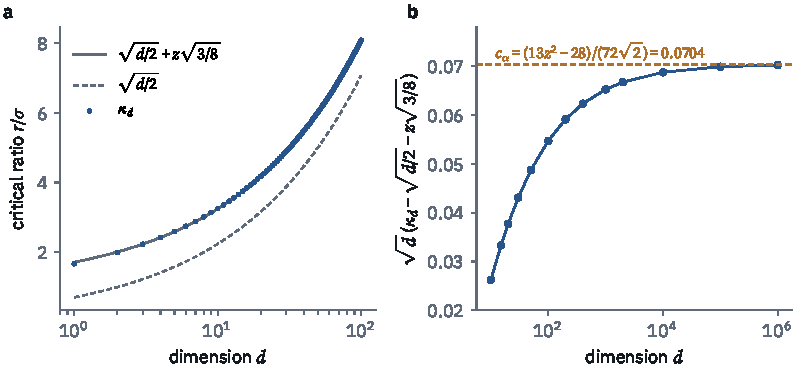
\includegraphics[width=\linewidth]{fig3_threshold.pdf}
\caption{(a) $\kappa_d$ at $\alpha = 0.05$ for $d = 1, \dots, 100$, against the two-term law
$\sqrt{d/2} + z\sqrt{3/8}$ and the leading term $\sqrt{d/2}$. The two-term law is within $10^{-2}$ from $d = 3$ on.
(b) The rescaled remainder $\sqrt d\,(\kappa_d - \sqrt{d/2} - z\sqrt{3/8})$ for $d = 10$ to $10^6$, converging to
$c_\alpha = 0.0704$ (Theorem~\ref{thm:main}(c)). Adding the third term improves on the two-term law only for
$d \ge 17$.}
\label{fig:threshold}
\end{figure}

\subsection{Beyond Gaussian noise}\label{sec:noise}

Let $r = \|x - a\| + \sigma\varepsilon$ where $\varepsilon$ has density $\propto e^{-V(|\varepsilon|)}$, and define
$M_d^V$ as $M_d$ with $(u - \kappa)^2/2$ replaced by $V(|u - \kappa|)$.

\begin{theorem}\label{thm:noise}
Let $V : [0,\infty) \to \R$ be continuous and strictly increasing, with
\begin{enumerate}[label=(\Alph*)]
\item[(C)] $t \mapsto V(e^t)$ strictly convex on $\R$, and
\item[(P)] $\int_0^\infty v^{d-1}e^{-V(v)}\dd v < \infty$.
\end{enumerate}
Then the posterior is proper, Lemma~\ref{lem:shell} holds with $M_d^V$, and there is a unique $\kappa_d^V(\alpha)$ such
that $\HPD$ has a hole if and only if $r/\sigma > \kappa_d^V(\alpha)$. For differentiable $V$, (C) holds whenever
$vV'(v)$ is strictly increasing.
\end{theorem}

\begin{proof}
Properness follows from (P) and $(v + \kappa)^{d-1} \le 2^{d-1}(v^{d-1} + \kappa^{d-1})$; superlevel sets are shells as
before, since $V$ is strictly increasing. Substituting $u = \kappa v$, the rescaled radius $v$ has density
$f_\kappa(v) \propto v^{d-1}e^{-V(\kappa|v-1|)}$ on $(0, \infty)$. For $\kappa < \kappa'$ and $y = |v - 1| > 0$,
\begin{gather*}
\frac{f_{\kappa'}}{f_\kappa}(v) = C\exp\bigl(-[V(\kappa'y) - V(\kappa y)]\bigr), \\
V(\kappa' y) - V(\kappa y) = \tilde V(\log y + \log\kappa') - \tilde V(\log y + \log\kappa),
\end{gather*}
with $\tilde V(t) = V(e^t)$. Increments of a strictly convex function over a fixed step increase strictly, so the likelihood
ratio $L$ is strictly decreasing in $y$: a monotone likelihood ratio \citep{karlin1956}. With $A = \{|v - 1| < 1\}$ and $E_\kappa L = 1$,
$\Pr_{\kappa'}(A) - \Pr_\kappa(A) = \Pr_\kappa(A)\Pr_\kappa(A^c)\bigl(E_\kappa[L \mid A] - E_\kappa[L \mid A^c]\bigr) > 0$: the same
sorting. Continuity is dominated convergence. As $\kappa \to 0$, the numerator of $M_d^V$ is at most
$e^{-V(0)}(2\kappa)^d/d \to 0$, while the denominator tends to $\int_0^\infty u^{d-1}e^{-V(u)}\dd u > 0$, by dominated
convergence with the bound $e^{-V(|u-\kappa|)} \le e^{-V(u/2)}$ for $u \ge 2\kappa$, which is integrable against $u^{d-1}$
by (P). As $\kappa \to \infty$ (take $\kappa \ge 2$), the numerator of $1 - M_d^V$ is
$\int_\kappa^\infty (v + \kappa)^{d-1}e^{-V(v)}\dd v \le 2^{d-1}\int_\kappa^\infty v^{d-1}e^{-V(v)}\dd v \to 0$ by (P), and
the denominator is at least $\int_{\kappa-1}^{\kappa+1} u^{d-1}e^{-V(|u-\kappa|)}\dd u \ge 2e^{-V(1)}$.
\end{proof}

No derivative of $V$ is used, so the theorem covers $V(v) = v^p$ for every $p > 0$, including $p < 1$ where $V'$ blows
up at $0$. \emph{Examples.} Exponential-power noise $V(v) = v^p$: $g(t) = e^{pt}$ is strictly convex. Laplace noise
($p = 1$) gives $M_1^V(\kappa) = 2(1 - e^{-\kappa})/(2 - e^{-\kappa})$ and $\kappa_1^V(\alpha) = \log\frac{1+\alpha}{2\alpha}$,
which is $\ln 10.5 = 2.351$ scale units, or $1.663$ standard deviations, at $\alpha = 0.05$ (Gaussian: $1.668$).
Student-$t$ noise with $\nu$ degrees of freedom: $vV'(v) = (\nu+1)v^2/(\nu + v^2)$ is increasing, and (P) holds if and
only if $\nu > d - 1$.

\begin{remark}[What carries over]\label{rem:carry}
Theorem~\ref{thm:main}(b) carries over when (P) also holds in dimension $d+1$, since its proof never uses the noise.
The growth law (c) does not, as the Laplace case shows.
\end{remark}

\begin{proposition}[Laplace noise]\label{prop:laplace}
For $V(v) = v$, let $q_d$ be the $(1-\alpha)$-quantile of the Gamma$(d,1)$ distribution. Then
$\kappa_d^V = q_d/2 + O(\sqrt d\,e^{-cd})$ for some $c > 0$, and so, in scale units,
\[ \kappa_d^V = \frac d2 + \frac z2\sqrt d + \frac{z^2 - 1}{6} + O(d^{-1/2}), \]
linear in $d$ rather than $\sqrt{d/2}$. At $\alpha = 0.05$: $\kappa_{50}^V = 31.087$ and $\kappa_{200}^V = 111.908$, against
$q_d/2 = 31.086$ and $111.908$.
\end{proposition}

\begin{proof}
Let $Y \sim \mathrm{Gamma}(d, 1)$ and $\varpi(\kappa) = \Pr(Y \le \kappa)$. Multiplying numerator and denominator of
$M_d^V(\kappa)$ by $e^{-\kappa}/\Gamma(d)$ turns the integrand into $u^{d-1}e^{-u}/\Gamma(d)$ on $u > \kappa$ and into
$u^{d-1}e^{u - 2\kappa}/\Gamma(d)$ on $u < \kappa$, whose integral $A = E[e^{2(Y-\kappa)};\, Y \le \kappa]$ lies in $[0, \varpi]$. So
\[ M_d^V(\kappa) = \frac{A + \Pr(\kappa < Y \le 2\kappa)}{A + \Pr(Y > \kappa)}, \]
and since $0 \le A \le \varpi$ and $\Pr(Y > \kappa) = 1 - \varpi$, this gives
$\Pr(Y \le 2\kappa) - \varpi \le M_d^V(\kappa) \le \Pr(Y \le 2\kappa)$. For $\kappa$ within $O(\sqrt d)$ of $d/2$, the Chernoff bound gives
$\varpi \le e^{-d(a - 1 - \log a)}$ with $a = \kappa/d \to 1/2$, and $\tfrac12 - 1 + \log 2 = 0.193 > 0$. Since $M_d^V$ is
increasing (Theorem~\ref{thm:noise}) and $\Pr(Y \le 2\kappa)$ has slope of order $d^{-1/2}$ near $\kappa = q_d/2$, the root of
$M_d^V = 1 - \alpha$ is within $O(\sqrt d\,e^{-cd})$ of $q_d/2$. The Cornish--Fisher expansion \citep{cornish1938} of the Gamma quantile, with mean
$d$, variance $d$ and skewness $2/\sqrt d$, is $q_d = d + z\sqrt d + (z^2 - 1)/3 + O(d^{-1/2})$.
\end{proof}

In the language of \S\ref{sec:high}: with Laplace noise the restoring force of the likelihood is constant rather than
linear in the residual, so the volume factor balances it at distance of order $d$, not $\sqrt d$. Existence of the
threshold is universal across the class of Theorem~\ref{thm:noise}; its growth law is specific to the noise.

\subsection{The mean is excluded}\label{sec:mean}

\begin{corollary}\label{cor:mean}
Under Gaussian noise, or the noise of Theorem~\ref{thm:noise} when $v^d e^{-V(v)}$ is integrable on $(0, \infty)$,
the posterior mean exists and equals $a$. Whenever $\HPD$ has a hole, the mean lies outside $\HPD$, at a strict local
minimum of the posterior density.
\end{corollary}

\begin{proof}
The reflection $x \mapsto 2a - x$ preserves $\|x - a\|$ and Lebesgue measure, so $X$ and $2a - X$ have the same law and
$E X = a$ when $E\|X\| < \infty$. Along every ray from $a$, $p \propto e^{-V((r - w)/\sigma)}$ for $0 \le w \le r$, which
increases strictly in $w$; so $p(x) > p(a)$ for $0 < \|x - a\| < r$.
\end{proof}

\begin{proposition}[Same two moments, different topology]\label{prop:gauss}
Assume Gaussian noise, or the noise of Theorem~\ref{thm:noise} with $\int_0^\infty v^{d+1}e^{-V(v)}\dd v < \infty$. Let
$\varsigma^2 = E\|X - a\|^2/d$ and $G = N(a, \varsigma^2I_d)$. Then $G$ and the posterior have the same mean and covariance,
every HPD region of $G$ is a ball, and for $r/\sigma > \kappa_d(\alpha)$ (Gaussian noise), respectively
$r/\sigma > \kappa_d^V(\alpha)$ (otherwise), the posterior's $\HPD$ has $\beta_{d-1} = 1$ ($d \ge 2$), respectively
$\beta_0 = 2$ ($d = 1$).
\end{proposition}

\begin{proof}
For orthogonal $Q$, $x \mapsto a + Q(x - a)$ preserves the posterior, so its covariance $\Sigma$ satisfies
$\Sigma = Q\Sigma Q^\top$ for all $Q \in O(d)$. Coordinate reflections give $\Sigma_{ij} = 0$ for $i \ne j$ and permutations
give equal diagonal entries, so $\Sigma = (\tr\Sigma/d)I = \varsigma^2I$. The mean matches by Corollary~\ref{cor:mean}; the topology
is Lemma~\ref{lem:shell}.
\end{proof}

More generally, any density with convex superlevel sets (Gaussian, unimodal elliptical, log-concave; \citealp{saumard2014}) has
contractible HPD regions, so no summary drawn from such a family can represent the hole, however its parameters are fitted.
Proposition~\ref{prop:gauss} is complementary to \citet[Theorem~2]{tommei2026}: it concerns holes ($\beta_{d-1}$)
rather than components, arises in a measurement model rather than a constructed pair, and holds at an explicit, sharp
threshold in every dimension. Nor is the threshold an instance of \citet[Theorem~3]{tommei2026}, because the posterior is not differentiable at the
anchor, and the anchor is exactly where the hole fills.

\begin{figure}[t]\centering
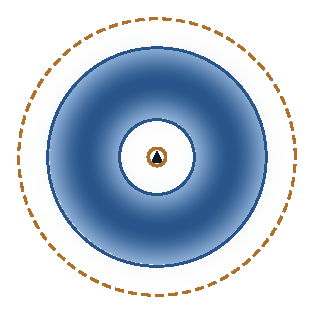
\includegraphics[width=.42\linewidth]{fig4_mean.pdf}
\caption{One range in the plane at $r/\sigma = 4$: the 95\% HPD ring, the posterior mean (open circle, at the anchor) in
its hole, and the 95\% region of the Gaussian with the same mean and covariance (dashed), a disc.}
\label{fig:mean}
\end{figure}

%======================================================================
\section{Two ranges}\label{sec:two}

Two anchors $a_1, a_2$ lie on the first coordinate axis, at coordinates $b_1 = -D/2$ and $b_2 = D/2$, and we observe
ranges $r_1, r_2$. We
assume that $D, r_1, r_2$ satisfy the strict triangle inequality, so that the two range spheres meet in a
$(d-2)$-sphere, the noise-free solution set, on which $S = 0$; exact data are not needed, and Lemma~\ref{rem:inconsistent} treats the other case.
Let $x^*$ be a noise-free solution of the observed ranges (it coincides with the true point only for exact data) and
$T$ the triangle $a_1 a_2 x^*$, with semiperimeter $s = (D + r_1 + r_2)/2$ and
incircle tangent lengths \citep{coxeter1969}
\[ t_* = s - D, \qquad t_1 = s - r_2, \qquad t_2 = s - r_1 \]
from $x^*$, $a_1$ and $a_2$. All three are positive, and $r_1 = t_* + t_1$, $r_2 = t_* + t_2$, $D = t_1 + t_2$. We write
$t_{\min} = \min(t_*, t_1, t_2)$.

\subsection{Reduction to a half-plane}

Write $x = (\xi, \rho\vartheta)$ with $\xi \in \R$, $\rho \ge 0$ the distance from the axis and $\vartheta \in S^{d-2}$, and
$w_i = \sqrt{(\xi - b_i)^2 + \rho^2}$ for the distance to $a_i$. Then $S = \sum_i (w_i - r_i)^2$ depends on $(\xi,\rho)$
only, and $\dd x = \rho^{d-2}\dd\xi\dd\rho\dd\vartheta$. Every HPD region is therefore the rotation about the axis of a region
$C$ in the closed half-plane $\bar\Omega = \{\rho \ge 0\}$, the closure of $\Omega = \{\rho > 0\}$, that is defined by $S$ alone; only its cut-off depends on $d$
(for $d = 2$, $S^0 = \{\pm1\}$ and rotation is reflection).

\begin{lemma}[Lift]\label{lem:lift}
Let $C \subset \bar\Omega$ be compact, connected and contractible, meeting the axis in $m$ disjoint closed intervals
(possibly points), with $(C, C \cap \partial\Omega)$ a finite CW pair, and let $X \subset \R^d$ be its rotation. If $m = 0$,
$X \simeq S^{d-2}$ (two contractible components if $d = 2$). If $m \ge 1$, $X \simeq \bigvee_{m-1} S^{d-1}$; in
particular $X$ is connected and $\beta_{d-1}(X) = m - 1$.
\end{lemma}

\begin{proof}
Let $k = d - 2$ and $A = C \cap \partial\Omega = A_1 \sqcup \dots \sqcup A_m$. Then $X = (C \times S^k)/\!\sim$, collapsing
the sphere over each point of $A$. If $m = 0$, $X \cong C \times S^k \simeq S^k$. If $m \ge 1$, $X$ is the pushout of
$A \leftarrow A \times S^k \hookrightarrow C \times S^k$. The inclusion is a cofibration, so this is a homotopy pushout and
each space may be replaced up to homotopy: $C \times S^k \simeq S^k$, $A_j \times S^k \simeq S^k$ included by a homotopy
equivalence, $A_j \simeq \mathrm{pt}$. So $X$ is $S^k$ with $m$ cones attached along the identity. The first cone gives a
contractible disc; each further cone is attached along a null-homotopic map and wedges on $\Sigma S^k = S^{k+1}$.
\end{proof}

\subsection{Residual coordinates}

The key change of variables replaces a point by its two range residuals $e_i = w_i - r_i$:
$\Psi(\xi, \rho) = (w_1 - r_1, w_2 - r_2)$ on $\bar\Omega$.

\begin{lemma}[Residual coordinates]\label{lem:residual}
\begin{enumerate}[label=(\roman*)]
\item $\Psi$ is a diffeomorphism of $\Omega$ onto the half-strip
\[ F = \{e \in \R^2 : e_1 + e_2 > -2t_*,\ \ e_1 - e_2 < 2t_2,\ \ e_2 - e_1 < 2t_1\}, \]
and extends to a homeomorphism $\bar\Omega \to \bar F$. It maps the segment $[a_1, a_2]$ onto the base edge
$\{e_1 + e_2 = -2t_*\}$, the ray beyond $a_2$ onto the edge $\{e_1 - e_2 = 2t_2\}$, the ray beyond $a_1$ onto the edge
$\{e_2 - e_1 = 2t_1\}$, and the anchors onto the two corners.
\item $S = |e|^2$, and for every rotation-invariant set $B$ with half-plane picture $B'$,
\[ \Pi_\sigma(B) = \frac{\int_{\Psi(B')} e^{-|e|^2/2\sigma^2} J(e)\dd e}{\int_F e^{-|e|^2/2\sigma^2} J(e)\dd e}, \qquad
   J = w_1 w_2\, h^{d-3}, \]
where $h = \rho$ is the height over the base $D$ of the triangle with sides $D, w_1, w_2$.
\item The edges lie on lines at distances $\sqrt2\,t_*$, $\sqrt2\,t_1$, $\sqrt2\,t_2$ from the origin, and the foot of
the perpendicular from $0$ lies in the relative interior of each edge. The corners $a_1, a_2$ lie at distances
$\sqrt{2(t_*^2 + t_1^2)}$ and $\sqrt{2(t_*^2 + t_2^2)}$.
\end{enumerate}
\end{lemma}

\begin{proof}
(i) From $w_1^2 - w_2^2 = 2\xi D$ we recover $\xi = (w_1^2 - w_2^2)/2D$, and then $\rho = (w_1^2 - (\xi + D/2)^2)^{1/2}$.
So $(w_1, w_2)$ determines $(\xi, \rho)$, and $\rho > 0$ is exactly the condition that $D, w_1, w_2$ form a
non-degenerate triangle: $w_1 + w_2 > D$ and $|w_1 - w_2| < D$. With $r_1 + r_2 - D = 2t_*$, $D + r_2 - r_1 = 2t_2$ and
$D + r_1 - r_2 = 2t_1$ these three conditions are the three inequalities defining $F$. The Jacobian is
\[ \det\frac{\partial(w_1, w_2)}{\partial(\xi, \rho)}
   = \frac{(\xi - b_1)\rho - (\xi - b_2)\rho}{w_1 w_2} = \frac{\rho D}{w_1 w_2} \ne 0 . \]
On the axis, $(w_1, w_2) = (|\xi + D/2|, |\xi - D/2|)$ is injective in $\xi$, and on the three stretches cut by the anchors
it satisfies $w_1 + w_2 = D$, $w_1 - w_2 = D$ and $w_2 - w_1 = D$ respectively. So the extension of $\Psi$ to $\bar\Omega$ is a
continuous bijection onto $\bar F$; it is proper, hence a homeomorphism.

(ii) $S = e_1^2 + e_2^2$ by definition, and by the Jacobian in (i) the posterior mass element in the half-plane is
\[ e^{-S/2\sigma^2}\rho^{d-2}\dd\xi\dd\rho = e^{-|e|^2/2\sigma^2}\,\frac{w_1w_2\,\rho^{d-3}}{D}\dd e ; \]
the constant $1/D$ cancels.

(iii) The line $e_1 + e_2 = -2t_*$ lies at distance $2t_*/\sqrt2$ from the origin, and similarly for the others. The feet
are $(-t_*, -t_*)$, $(t_2, -t_2)$ and $(-t_1, t_1)$; the first has $e_1 - e_2 = 0 \in (-2t_1, 2t_2)$, and the other two
have $e_1 + e_2 = 0 > -2t_*$, so each lies inside its edge. The corner on the $t_2$-edge is
$(t_2 - t_*, -t_2 - t_*)$, where $w_2 = r_2 - t_2 - t_* = 0$: it is $a_2$, at squared distance $2(t_*^2 + t_2^2)$.
\end{proof}

So in residual coordinates the posterior is an isotropic Gaussian times the weight $J$ on a half-strip, and since
$\Delta = |e|^2/2$, \emph{every HPD region is a disc, $\{|e|^2 \le 2\Delta_\alpha(\sigma)\}$, cut by the walls of $F$}
(Figure~\ref{fig:residual}). The dimension enters only through $J$, and therefore only through the cut-off.


\subsection{The triangle theorem}

\begin{theorem}[Triangle theorem]\label{thm:triangle}
Off the axis, the only critical points of $S$ are the noise-free solutions. On the axis, $f(\xi) = S(\xi, 0)$ has exactly
three local minima:
\begin{itemize}[leftmargin=1.2em]
\item the inner point $\xi = (r_1 - r_2)/2$, where the incircle of $T$ touches $a_1a_2$, at depth $t_*^2$;
\item the outer point $\xi = -D/2 - t_*$, where the excircle opposite $a_2$ touches the line, at depth $t_1^2$;
\item the outer point $\xi = D/2 + t_*$, where the excircle opposite $a_1$ touches the line, at depth $t_2^2$.
\end{itemize}
Its local maxima are the anchors, at depths $t_*^2 + t_1^2$ and $t_*^2 + t_2^2$; they are strict local maxima of $S$ in
$\R^d$. The three smooth points are non-degenerate saddles of $S$ of index $d - 1$.
\end{theorem}

\begin{proof}
Off the axis, $S$ is a smooth function of $(\xi, \rho)$, and $S \circ \Psi^{-1} = |e|^2$ has the single critical point
$e = 0$ in $F$, which is $x^*$. On the axis, $\Psi$ is affine on each stretch with speed $\sqrt 2$, so $f$ restricted
to a stretch is the squared distance from the origin along a line: a convex quadratic with its minimum at the foot of
the perpendicular, at depth $\tfrac12(\text{wall distance})^2$. By Lemma~\ref{lem:residual}(iii) the three feet lie inside
their edges, at depths $t_*^2, t_1^2, t_2^2$, and $f$ increases from both feet towards each corner, so the corners are
the local maxima, at depths $t_*^2 + t_i^2$. The feet are, in the plane, the points with $w_1 = r_1 - t_* = t_1$ on the
segment and with $(w_1, w_2) = (t_*, s)$ and $(s, t_*)$ on the rays; these are the stated touch points, since the
excircle opposite $a_2$ touches the line $a_1a_2$ at distance $s$ from $a_2$.

Near an axis point $(\xi, 0)$ with $w_i = |\xi - b_i| > 0$, $\sqrt{(\xi - b_i)^2 + \rho^2} = w_i + \rho^2/2w_i + O(\rho^4)$,
so $S(\xi, \rho) = f(\xi) + \rho^2\sum_i e_i/w_i + O(\rho^4)$ with $e_i = w_i - r_i$. At the inner point $e_i = -t_*$; at the point beyond $a_2$,
$e = (t_2, -t_2)$ and $w = (s, t_*)$, so $\sum_i e_i/w_i = -t_2 D/(st_*)$; symmetrically beyond $a_1$. All are negative,
while $f'' = 4$: the Hessian of $S$ has one positive and $d-1$ negative eigenvalues. At $a_1$, along any unit direction
$\vartheta$, $S(a_1 + t\vartheta) - S(a_1) \le -2t\bigl(r_1 - |D - r_2|\bigr) + O(t^2)$, and $r_1 > |D - r_2|$ by the
strict triangle inequality.
\end{proof}

Each smooth critical depth is a squared incircle tangent length, and each anchor depth is the sum of two of them
(Figure~\ref{fig:triangle}). The proof also explains the incircle: between the anchors $w_1 + w_2 = D$, so the total
shortfall $e_1 + e_2 = -2t_*$ is fixed and $e_1^2 + e_2^2$ is smallest when the two shortfalls are equal, which is the
equal-tangent property of the incircle; beyond an anchor $|w_1 - w_2| = D$ is fixed instead, and the minimiser overshoots
one sphere by as much as it falls short of the other, the equal-tangent property of an excircle.

\begin{figure}[t]\centering
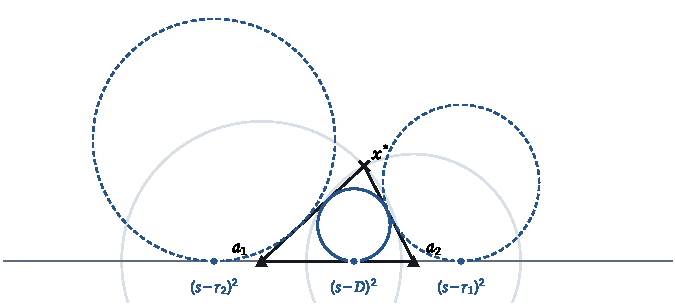
\includegraphics[width=.86\linewidth]{fig5_triangle.pdf}
\caption{The triangle theorem. The three smooth critical points of $S$ on the anchor line are where the incircle (solid)
and the two excircles on the side of $x^*$ (dashed) touch it; their depths are the squared tangent lengths
$(s - r_2)^2 = t_1^2$, $(s - D)^2 = t_*^2$, $(s - r_1)^2 = t_2^2$. Grey: the two range circles.}
\label{fig:triangle}
\end{figure}

\subsection{The whole sequence of topologies}

\begin{proposition}[Everything happens on the axis]\label{prop:axis}
For $\delta \ge 0$ let $C_\delta = \{\Delta \le \delta\} \cap \bar\Omega$ and
\[ m(\delta) = \#\{k \in \{*, 1, 2\} : t_k^2 \le \delta\} - \#\{i \in \{1, 2\} : t_*^2 + t_i^2 \le \delta\}. \]
Then $C_\delta$ is compact, connected and contractible, and meets the axis in exactly $m(\delta)$ closed intervals.
Consequently the HPD region, the rotation of $C_{\Delta_\alpha(\sigma)}$, is described by Lemma~\ref{lem:lift} with
$m = m(\Delta_\alpha(\sigma))$: for $m = 0$ it has the noise-free topology (two contractible pieces for $d = 2$, a tube
$\simeq S^{d-2}$ for $d \ge 3$); for $m \ge 1$ it is connected with $\beta_{d-1} = m - 1$ and no other homology.
\end{proposition}

\begin{proof}
By Lemma~\ref{lem:residual}, $\Psi(C_\delta) = \{|e| \le \sqrt{2\delta}\} \cap \bar F$, an intersection of a disc and a closed
convex set: compact, convex, hence contractible and connected. Its trace on $\partial F$ is the trace of the disc on a
polygonal path with three edges and two corners. Each edge meets the disc in an interval, non-empty if and only if the
edge's distance from $0$, which is its wall distance because the foot lies inside it, is at most $\sqrt{2\delta}$; two
consecutive non-empty intervals join if and only if their common corner lies in the disc. A path has no cycles, so the
number of components is the number of edges met minus the number of corners met. This is $m(\delta)$ by
Lemma~\ref{lem:residual}(iii). For $\delta > 0$ the convex set $\Psi(C_\delta)$ has the origin in its interior, so radial
projection from the origin is a homeomorphism onto a closed disc carrying its boundary onto the circle and the trace on
$\partial F$ onto $m(\delta)$ disjoint closed arcs or points; a disc with finitely many boundary arcs is a finite CW pair.
$\Psi$ transfers everything to $C_\delta$, and for $\delta = 0$, $C_0 = \{x^*\}$.
\end{proof}

By Theorem~\ref{thm:depth}, $\Delta_\alpha(\sigma)$ sweeps $(0, \infty)$ continuously and increasingly, so as the noise
grows the region steps through $m = m(\delta)$, one step per crossing, in every dimension. A contact ($\delta = t_k^2$)
raises $m$ by one and an anchor ($\delta = t_*^2 + t_i^2$) lowers it by one (Figures~\ref{fig:ladder}
and~\ref{fig:phase}).

\begin{corollary}[Which breaks first]\label{cor:first}
Suppose $t_*, t_1, t_2$ are distinct. In every dimension $d \ge 2$:
\begin{enumerate}[label=(\roman*)]
\item the first transition is a merge ($m: 0 \to 1$): the two pieces join ($d = 2$), the tube fills ($d \ge 3$). It
happens between the anchors if $D$ is the longest side of $T$, and otherwise around the outside, beyond the anchor
nearer $x^*$;
\item the second transition creates a cavity ($m: 1 \to 2$): a ring ($d = 2$), a hollow shell ($d \ge 3$);
\item two cavities coexist at some noise level if and only if $D\,|r_1 - r_2| < t_*^2$.
\end{enumerate}
\end{corollary}

\begin{proof}
Each anchor depth $t_*^2 + t_i^2$ exceeds two of the three contact depths, hence the second smallest. So the first two
events are contacts, which gives (i) and (ii) with Lemma~\ref{lem:lift}; the smallest tangent length belongs to the
vertex opposite the longest side. For (iii), $m = 3$ at some $\delta$ if and only if all three contacts precede both
anchors, i.e.\ $\max(t_1^2, t_2^2) < t_*^2 + \min(t_1^2, t_2^2)$, i.e.\ $|t_1^2 - t_2^2| < t_*^2$; and
$t_1^2 - t_2^2 = (t_1 - t_2)(t_1 + t_2) = (r_1 - r_2)D$.
\end{proof}

When $r_1 = r_2$ the two outer contacts coincide: for crossing angle $\angle a_1x^*a_2 < 60^\circ$ the two pieces become a
ring in one step ($m: 0 \to 2$), and at $60^\circ$ all three contacts coincide. For the asymmetric example $D = 2$,
$x^* = (0.2, 1.1)$, the depths are $t_*^2 = 0.244$, $t_2^2 = 0.750$, $t_*^2 + t_2^2 = 0.994$, $t_1^2 = 1.286$ and
$t_*^2 + t_1^2 = 1.530$, so at 95\% in the plane the region goes two pieces $\to$ one $\to$ ring $\to$ one $\to$ ring
$\to$ one, at $\sigma = 0.282$, $0.517$, $0.609$, $0.708$ and $0.790$ (Figure~\ref{fig:ladder}). More noise first creates
holes and then removes them. In space the same steps produce cavities (Figure~\ref{fig:ladder3d}): for a symmetric
triangle with crossing angle $45^\circ$ the tube becomes a shell with one cavity, which splits into two around the
anchors and then fills.

\begin{figure}[t]\centering
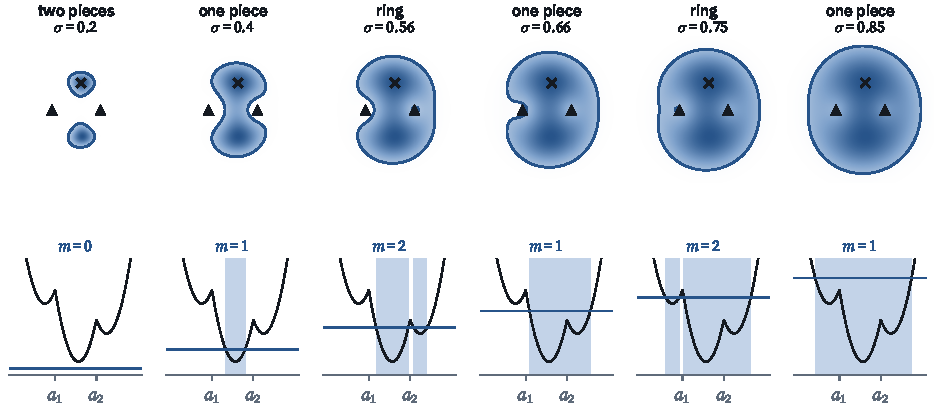
\includegraphics[width=\linewidth]{fig6_axis_ladder.pdf}
\caption{The sequence of topologies for $D = 2$, $x^* = (0.2, 1.1)$, $d = 2$, as the noise rises. Top: the 95\% HPD
region. Bottom: the axis profile $f$ with the HPD cut-off (horizontal line); the shaded intervals are the trace of the
region on the axis, and their number $m$ determines the topology (Proposition~\ref{prop:axis}). The first hole forms
around $a_2$, the second around $a_1$.}
\label{fig:ladder}
\end{figure}

\begin{figure}[t]\centering
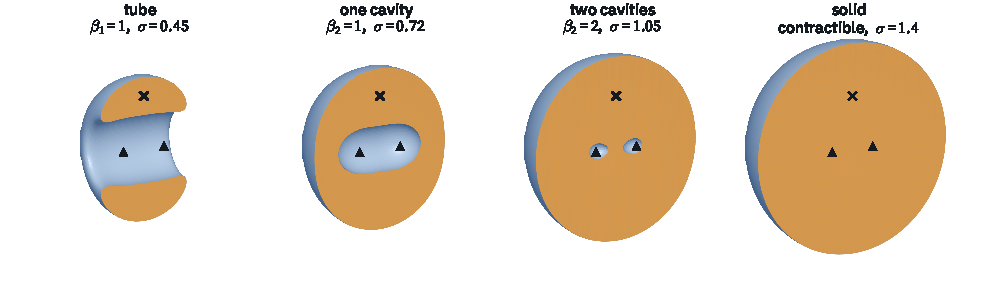
\includegraphics[width=\linewidth]{fig12_ladder_3d.pdf}
\caption{The backwards staircase in space ($d = 3$): two ranges, anchors at $\pm1$, crossing angle $45^\circ$, 95\% HPD
regions cut open along the plane through the anchors and the true point (amber: cut face). As the noise rises the tube
($\sigma < 0.61$) becomes a shell with one cavity around the segment $a_1a_2$ ($0.61 < \sigma < 1.03$), the cavity splits
into two around the anchors ($1.03 < \sigma < 1.20$), and the region fills ($\sigma > 1.20$). Here the outer contacts
come first ($\theta < 60^\circ$), so $m$ runs $0 \to 2 \to 3 \to 1$.}
\label{fig:ladder3d}
\end{figure}

\begin{figure}[t]\centering
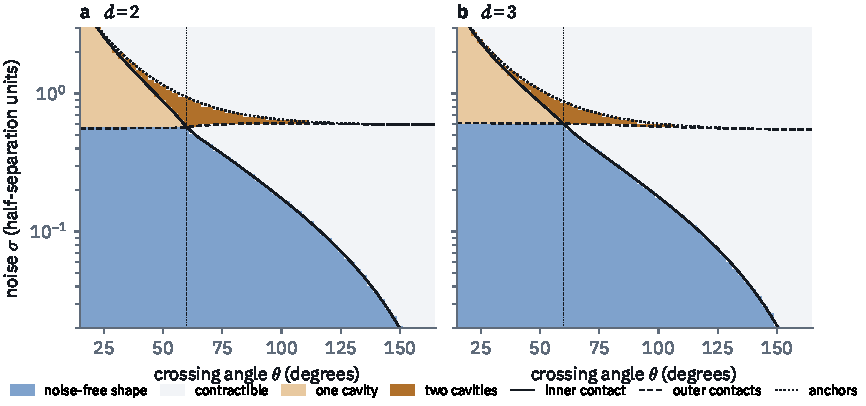
\includegraphics[width=\linewidth]{fig7_phase.pdf}
\caption{Symmetric geometry ($r_1 = r_2$, anchors at $\pm1$): topology of the 95\% region computed by brute force over
crossing angle and noise (colours), with the transition curves predicted by Theorems~\ref{thm:depth}
and~\ref{thm:triangle} (black), for $d = 2$ and $d = 3$. They coincide. The order of events switches at $60^\circ$.}
\label{fig:phase}
\end{figure}

\begin{figure}[t]\centering
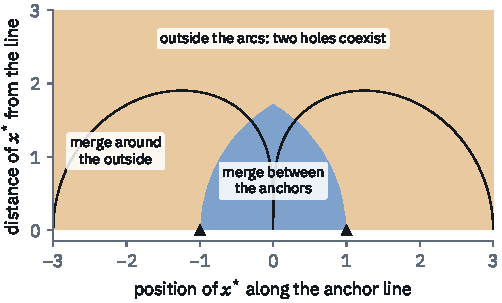
\includegraphics[width=.66\linewidth]{fig8_first_event.pdf}
\caption{Which event comes first, over all positions of $x^*$ (anchors at $\pm1$). Blue: the pieces first merge between
the anchors ($D$ is the longest side of $T$); amber: around the outside. Two holes coexist at some noise level exactly
where $D|r_1 - r_2| < t_*^2$: outside the black curves, which includes a thin wedge around the symmetry line.}
\label{fig:firstevent}
\end{figure}

\begin{lemma}[Inconsistent data]\label{rem:inconsistent}
Suppose the observed $D, r_1, r_2$ violate the strict triangle inequality. Then every HPD region is connected and meets
the anchor line, so it never has the noise-free topology. If $r_1 + r_2 \le D$ it is contractible at every noise level.
If $r_1 + r_2 > D$ and $r_1 \ge r_2 + D$ (the case $r_2 \ge r_1 + D$ is symmetric), it is contractible, then has one hole
($d = 2$) or cavity ($d \ge 3$), then is contractible again.
\end{lemma}

\begin{proof}
The proof of Lemma~\ref{lem:residual}(i) does not use the ranges: $(\xi, \rho) \mapsto (w_1, w_2)$ is a homeomorphism of
$\bar\Omega$ onto the closed convex set $\bar G = \{w_1 + w_2 \ge D,\ |w_1 - w_2| \le D\}$, carrying the axis onto $\partial G$,
the anchors onto the corners $(0, D)$ and $(D, 0)$, and the segment and the two rays onto the three edges. In these
coordinates $S = |w - r|^2$ with $r = (r_1, r_2) \notin G$. So every sublevel set is a disc centred at $r$ cut by
$\bar G$: it is convex, and once non-empty it contains the point of $\bar G$ nearest to $r$, which lies on $\partial G$,
that is, on the axis. The proof of Proposition~\ref{prop:axis} then applies with the disc centred at $r$ instead of the
origin (radial projection from any interior point), so the region is described by Lemma~\ref{lem:lift} with $m \ge 1$:
it is connected and never $\simeq S^{d-2}$.

Write $m = [B] + [E_1] + [E_2] - [a_1] - [a_2]$, where $B$ is the base edge, $E_i$ the ray beyond $a_i$, and $[\,\cdot\,]$
is $1$ if the disc meets the edge or contains the corner. An edge whose foot of the perpendicular from $r$ lies at or
beyond one of its corners is met exactly when that corner is contained. If $r_1 + r_2 \le D$, the projection of
$r - (D, 0)$ on the direction $(1, 1)$ of $E_2$ is $(r_1 + r_2 - D)/2 \le 0$, and likewise at $(0, D)$; so
$[E_i] = [a_i]$, and $m = [B] = 1$ throughout. If $r_1 + r_2 > D$ and $r_1 \ge r_2 + D$, the feet on $E_1$ and $E_2$ lie on
them, the foot on the base has first coordinate $(D + r_1 - r_2)/2 \ge D$, at or beyond $a_2$, so $[B] = [a_2]$, and
$m = [E_2] + [E_1] - [a_1]$. The disc meets $E_2$ first, since $r$ lies beyond its line, and $E_1$ before it contains
$a_1$, so $m$ runs $1 \to 2 \to 1$.
\end{proof}

Either way the two-piece phase, flip ambiguity, is absent: the region looks unambiguous because the data are
inconsistent, not because the flip has been resolved.

\subsection{Three ranges in the plane}\label{sec:three}

With three non-collinear anchors in $\R^2$, three unit vectors are always linearly dependent, so $S$ may have critical
points with non-zero residuals, and residual coordinates no longer straighten the problem.

\begin{remark}[Holes and maxima]\label{rem:three}
Along a ray from $a_i$, $S(a_i + t\vartheta) - S(a_i) = -2t(r_i - v_i\cdot\vartheta) + O(t^2)$ with
$v_i = \sum_{j \ne i}(\|a_i - a_j\| - r_j)u_{ij}$, where $u_{ij}$ is the unit vector from $a_j$ to $a_i$; so $a_i$ is a
strict local minimum of $p$ if $r_i > |v_i|$, and not a local minimum if $r_i < |v_i|$. In the plane,
$\beta_1(\{S \le c\})$ counts the bounded components of $\{S > c\}$, each of which contains a local maximum of $S$, and
the cut-off sweeps all levels; so the HPD region has a hole at some noise level if and only if $S$ has a local maximum,
at an anchor or a smooth one. A smooth one requires $\sum_i r_i/w_i \ge 6$, since the trace of the Hessian is
$12 - 2\sum_i r_i/w_i$. For the equilateral anchors $(0, 1)$ and $(\pm\sqrt3/2, -1/2)$, no anchor qualifies when $x^*$
is the centre, all three do at $x^* = (0, -2.5)$ (where the 95\% region has a hole for $\sigma \approx 0.96$--$1.67$),
and exactly one does at $(2.5, 1.5)$.
\end{remark}

When the truth is far from the anchors the picture is complete, and it has a hole that surrounds no anchor. Let $x_F$
be the Fermat point of the anchors, the minimiser of the total distance $\mathcal D(x) = \sum_i\|x - a_i\|$; let $\bar a$ be
their centroid and $M = \sum_i(a_i - \bar a)(a_i - \bar a)^\top$, with eigenvalues $\lambda_1 \ge \lambda_2 > 0$; and for a
unit vector $\vartheta_*$, the direction of the truth, put $G(\vartheta) = (\vartheta_* - \vartheta)^\top M(\vartheta_* - \vartheta)$ for
unit vectors $\vartheta$.

\begin{theorem}[Far truth]\label{thm:far}
Let the data be exact, with $x^* = \varrho\,\vartheta_*$, the anchors fixed, and $\varrho \to \infty$; assume that the critical
points of $G$ on the unit circle are non-degenerate.
\begin{enumerate}[label=(\roman*)]
\item If every angle of the anchor triangle is less than $120^\circ$, $S$ has a non-degenerate local maximum $x_\varrho$
with $x_\varrho - x_F = O(1/\varrho)$ and $\Delta(x_\varrho) > \Delta(a_i)$ for every $i$, and no anchor is a local maximum of $S$.
If one angle exceeds $120^\circ$, the anchor at that vertex is a local maximum, and $S$ has no smooth critical point
within a fixed distance of the anchors.
\item Outside a fixed disc around the anchors, the critical points of $S$ lie at distance $\varrho + O(1)$ from the origin,
in directions that tend to the critical points of $G$: a minimum of $G$ gives a local minimum of $S$, a maximum gives a
saddle, and the depth tends to $\frac12 G$ there. $G$ has two critical points, or four exactly when
$(\lambda_1|\vartheta_{*1}|)^{2/3} + (\lambda_2|\vartheta_{*2}|)^{2/3} < (\lambda_1 - \lambda_2)^{2/3}$, with $\vartheta_{*k}$ the
coordinates of $\vartheta_*$ along the eigenvectors of $M$; four needs $\lambda_1 > 2\lambda_2$.
\item Hence, if every angle is below $120^\circ$ and $G$ has two critical points, $S$ has exactly three critical points,
$x^*$, a saddle and $x_\varrho$, and for $d = 2$ the HPD region is contractible while $\Delta_\alpha$ is below the depth of
the saddle, which tends to $\frac12\max G$; a ring around the anchors from that depth until $\Delta_\alpha$ reaches
$\Delta(x_\varrho) = \frac12\sum_i(r_i - \|x_F - a_i\|)^2 + O(1/\varrho)$; and contractible again beyond.
\end{enumerate}
\end{theorem}

The proof is in Supplement~\ref{app:three}. Its core is the expansion
$S = \sum_i r_i^2 - 2\varrho\,\mathcal D(x) + O(1)$ near the anchors: the least plausible point of the cluster is the one with
the smallest total distance to the anchors. Seen from far away, three ranges are three nearly equal measurements of one
distance, and the region behaves like that of a single range whose anchor is the Fermat point (Figure~\ref{fig:three}).
The threshold of Theorem~\ref{thm:main} carries over approximately: for $x^* = (0, -8)$ and the equilateral anchors above,
the hole forms at $\sigma = 0.969$ and closes at $\sigma = 6.167$, against $\sqrt{2\Delta(x_\varrho)}/\kappa_2 = 6.137$. When $G$
has four critical points, $S$ has a second local minimum far away. For the anchors $(\pm2, 0)$, $(0, 1.5)$,
$\vartheta_* = (0, -1)$ and $\varrho = 60$, it lies at $(0, 61.0007)$, at depth $2.999$ against the limit $2\lambda_2 = 3$; as the
anchors become collinear it tends to the mirror image of $x^*$ in their line, at depth $2\lambda_2 \to 0$. It is what
remains of the flip ambiguity, and it can split the region: for $x^* = (0, -20)$ the $95\%$ region is two pieces at
$\sigma = 1$, a false flip ambiguity although three ranges determine the point.

\begin{figure}[t]\centering
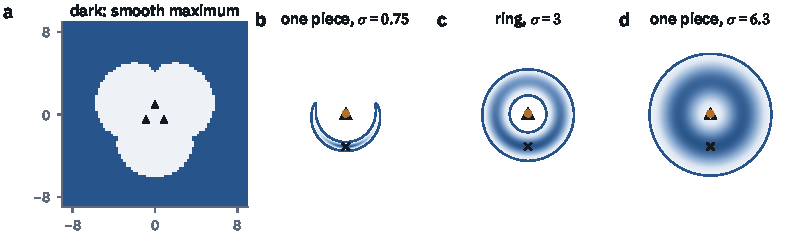
\includegraphics[width=\linewidth]{fig14_three.pdf}
\caption{Three ranges in the plane, anchors $(0, 1)$, $(\pm\sqrt3/2, -1/2)$ (triangles), exact data. (a) Positions of
$x^*$ at which $S$ has a smooth local maximum (dark): only when the truth is far from the anchors. (b)--(d) $x^* = (0, -8)$
(cross): the $95\%$ region is an arc, then a ring around all three anchors, then one piece; the hole closes at the smooth
maximum (amber, at the Fermat point up to $O(1/\varrho)$), at $\sigma = 6.167$, after every anchor has been covered
(Theorem~\ref{thm:far}). Each panel's Betti numbers were checked on the grid.}
\label{fig:three}
\end{figure}

\begin{proposition}[How the Fermat maximum is born]\label{prop:birth}
Take the anchors $(0, 1)$, $(\pm\sqrt3/2, -1/2)$, exact data with $x^* = (0, -\varrho)$, and $\varrho \ge 2$. The anchor $(0, 1)$
is a local maximum of $S$ exactly for $\varrho < 13/2$, and the other two exactly for $\varrho < 2.7227$. On the symmetry
axis inside the triangle, $S$ has no critical point for $\varrho < \varrho_0 = (1 + 5\sqrt5)/2 = 6.0902$; at $\varrho_0$ a
degenerate one appears at $(0, (\sqrt5 - 1)/2)$ and splits into a strict local maximum and a saddle. The saddle reaches
$(0, 1)$ at $\varrho = 13/2$, exactly when that anchor stops being a local maximum, and the maximum tends to the centre,
the Fermat point, as $\varrho \to \infty$.
\end{proposition}

So the hole that closes at an anchor for nearby truths and the one that closes at the Fermat point for distant truths
are exchanged through a fold, at a golden-ratio point of the axis. Not every exchange is a fold. Along a ray from $a_i$,
$S(a_i + t\vartheta) = S(a_i) - 2t(r_i - v_i\cdot\vartheta) + c\,t^2 + O(t^3)$; when $c < 0$ in the direction of $v_i$ at the
moment the test fails, as on an isosceles triangle with a $115^\circ$ apex, the anchor releases a smooth maximum
directly, at distance $(|v_i| - r_i)/|c|$ from itself. With noise $\sigma\omega_i$ on range $i$, the same argument puts the
last hole at the minimiser of $\sum_i\|x - a_i\|/\omega_i^2$. Two questions remain open. A smooth maximum can occur even
when $x^*$ is inside the anchor triangle: for the anchors $(2.2308, -0.2168)$, $(-1.2836, -3.3176)$, $(2.0261, 0.0052)$
and $x^* = (1.0874, -1.1301)$, $S$ has a strict local maximum at $(2.2112, -0.0204)$, between the two anchors $0.30$
apart, so what matters is the distance of the truth relative to the anchor spacing it sees. And in $30\,000$ random
configurations, with exact and with noisy data, $S$ never had more than one smooth local maximum ($4738$ had one); we
conjecture that this holds in general, which would make the complete sequence of topologies for three ranges in the
plane a finite case analysis. It fails for four anchors: two tight pairs, such as $(2.4153, -0.1525)$, $(2.4712, 0.0281)$
and $(-3.478, 1.7811)$, $(-3.2678, 1.3587)$ with $x^* = (-1.0069, -1.0872)$, each act as a small far cluster, and $S$ has
two strict smooth maxima.

\subsection{Up to $d$ ranges}\label{sec:nranges}

\begin{lemma}[Anchors in a subspace]\label{lem:subspace}
Let the anchors span an affine subspace $\mathcal A \ne \R^d$, and let the data be exact with a noise-free solution $x^* \notin \mathcal A$.
At every critical point $x_c \in \mathcal A$ of $S$ other than an anchor, $S$ has a strict transverse maximum: its second derivative
in every direction normal to $\mathcal A$ is negative. If moreover the anchors are affinely independent, every component of every
HPD region with an interior point contains a noise-free solution: no piece of a credible region is ever born on $\mathcal A$.
\end{lemma}

\begin{proof}
Let $u_i$ be the unit vector from $a_i$ to $x_c$, so $\sum_i e_iu_i = 0$. Write $x^* - x_c = q + \mu n$ with $q$ parallel to
$\mathcal A$, $n$ a unit normal and $\mu > 0$, and put $c = |q|^2 + \mu^2 > 0$. Then $A_i := r_i^2 - w_i^2 = 2w_iu_i\cdot q + c$,
so $e_i = -A_i/(r_i + w_i)$ and $u_i\cdot q = (A_i - c)/2w_i$. Taking the inner product of $\sum_i e_iu_i = 0$ with $q$,
\[ \sum_i \frac{A_i^2}{w_i(r_i + w_i)} = c\sum_i \frac{A_i}{w_i(r_i + w_i)} . \]
Not all $A_i$ vanish, since otherwise $x_c \in \mathcal A$ would have the same distances to the anchors as $x^* \notin \mathcal A$. So the
right-hand sum is positive, and the second derivative of $S$ in every normal direction is negative:
\[ 2\sum_i \frac{e_i}{w_i} = -2\sum_i \frac{A_i}{w_i(r_i + w_i)} < 0 . \]
For the second statement, let $K$ be a component of $\{S \le \lambda\}$ with an interior point and $x_0$ a minimiser of
$S$ on $K$. If $S(x_0) = \lambda$, $S$ would be constant on an open set, which a non-constant real-analytic function is not; so
$S(x_0) < \lambda$, a ball about $x_0$ lies in $K$, and $x_0$ is a local minimum of $S$.
Off $\mathcal A$ the vectors $x - a_i$ are linearly independent, so $\nabla S = 2\sum_i e_iu_i = 0$ forces $e = 0$. On $\mathcal A$ a smooth
local minimum would be a critical point of $S$, excluded by the first statement, and an anchor is never a local minimum,
since along $\vartheta = -v_i/|v_i|$ (any $\vartheta$ if $v_i = 0$) the slope of $S$ is $-2(r_i + |v_i|) < 0$, with $v_i$ as in
Remark~\ref{rem:three}.
\end{proof}

For two ranges, Lemma~\ref{lem:subspace} recovers the transverse part of Theorem~\ref{thm:triangle} without computing
the critical points. For three anchors in $\R^3$ the residual domain, the set of $e$ for which the ranges $r + e$ are realised
above the anchor plane (a Cayley--Menger condition; \citealp{blumenthal1953,liberti2014}), is not convex, so Proposition~\ref{prop:axis} does not carry over as it stands, and the contact set on the plane is a
union of patches rather than intervals. The noise-free regime, however, is settled for any number of ranges up to $d$.

\begin{theorem}[Up to $d$ ranges]\label{thm:nranges}
Let $a_1, \dots, a_n \in \R^d$, $1 \le n \le d$, be affinely independent with affine hull $\mathcal A$, let the observed
ranges be realised by a point $x^* \notin \mathcal A$, and let $\Delta_{\mathcal A} = \min_{\mathcal A}\Delta$. Then
$\Delta_{\mathcal A} > 0$, and:
\begin{enumerate}[label=(\roman*)]
\item if $\Delta_\alpha(\sigma) < \Delta_{\mathcal A}$, then $\HPD \cong B^n \times S^{d-n}$, where $B^n$ is the closed
$n$-ball; for $n = d$ it is two disjoint closed balls;
\item if $n = d$ and $\Delta_\alpha(\sigma) \ge \Delta_{\mathcal A}$, then $\HPD$ is connected.
\end{enumerate}
For $n = 1$, $\Delta_{\mathcal A} = r^2/2$ and (i) is the hole case of Lemma~\ref{lem:shell}; for $n = 2$,
$\Delta_{\mathcal A} = t_{\min}^2$ and (i) is the `if' half of Proposition~\ref{prop:criterion} below.
\end{theorem}

\begin{proof}
Write $x = (p, \rho\vartheta)$ with $p \in \mathcal A$, $\rho \ge 0$ the distance from $\mathcal A$ and
$\vartheta \in S^{d-n}$. Then $w_i = (|p - a_i|^2 + \rho^2)^{1/2}$, so $\Delta$ depends on $(p, \rho)$ only. On
$\Omega = \{\rho > 0\}$ the map $\Psi(p, \rho) = (w_i - r_i)_{i \le n}$ is injective: $w_i^2 - w_1^2 =
|p - a_i|^2 - |p - a_1|^2$ is affine in $p$ with linear part $2p\cdot(a_1 - a_i)$, and the $a_i - a_1$ span the
directions of $\mathcal A$, so $w$ determines $p$ and then $\rho$. Its Jacobian has rows $(p - a_i, \rho)/w_i$, the
vectors $(x - a_i)/w_i$, which are linearly independent because $x \notin \mathcal A$. So $\Psi$ is a local
diffeomorphism, and $\Delta = |\Psi|^2/2$ on $\Omega$. The minimum of $\Delta$ on $\mathcal A$ is attained, at $p_0$
say. Write $x^* = (p^*, \rho^*)$ with $\rho^* > 0$. If $\Delta(p_0) = 0$, then
$|p_0 - a_i|^2 = |p^* - a_i|^2 + \rho^{*2}$ for every $i$; subtracting these in pairs gives
$(p^* - p_0)\cdot(a_i - a_1) = 0$, so $p_0 = p^*$ and $\rho^* = 0$, a contradiction. Hence $\Delta_{\mathcal A} > 0$.

(i) $\Psi$ extends continuously to $\bar\Omega$ and is proper, so every boundary point of the open set $\Psi(\Omega)$
lies in $\Psi(\mathcal A)$, at distance at least $(2\Delta_{\mathcal A})^{1/2}$ from $0$. The ball
$B = \{|e|^2 \le 2\Delta_\alpha\}$ is connected, contains $\Psi(x^*) = 0$ and misses $\Psi(\mathcal A)$, so it lies in
$\Psi(\Omega)$. The half-space picture $C$ of $\HPD$ misses $\mathcal A$, where $\Delta \ge \Delta_{\mathcal A} > \Delta_\alpha$,
so $C \subset \Omega$ and $\Psi(C) = B$; and $\Psi$ restricted to the compact set $C$ is a continuous bijection onto $B$,
hence a homeomorphism onto $B \cong B^n$. As $\rho > 0$ on $C$, the map $((p, \rho), \vartheta) \mapsto (p, \rho\vartheta)$ is a
continuous bijection of $C \times S^{d-n}$ onto $\HPD$, hence a homeomorphism.

(ii) Now $\mathcal A$ is a hyperplane, and the reflection $\mathcal R$ in it preserves $\Delta$. Off
$\mathcal A$ the vectors $x - a_i$ are linearly independent, so $\nabla S = 2\sum_i e_i(x - a_i)/w_i = 0$ forces $e = 0$, and the
only critical points of $S$ off $\mathcal A$ are $x^*$ and $\mathcal Rx^*$. On $\mathcal A$ there is no local
minimum, by Lemma~\ref{lem:subspace} and its proof. Let $\delta' > \Delta_{\mathcal A}$ be a regular value of $\Delta$
that is not the depth of an anchor; such values are dense, by Sard's theorem. On a component $K$ of
$\{\Delta \le \delta'\}$, $\Delta$ attains its minimum at some $y$. If $\Delta(y) = \delta'$, then $\nabla\Delta(y) \ne 0$
and $K$ contains points near $y$ of smaller depth; so $\Delta(y) < \delta'$, $y$ is a local minimum of $\Delta$, and
$y \in \{x^*, \mathcal Rx^*\}$. Hence $\{\Delta \le \delta'\}$ has at most two components. The one containing
$p_0$ is mapped to itself by $\mathcal R$, which fixes $p_0$, so it contains both $x^*$ and
$\mathcal Rx^*$, and $\{\Delta \le \delta'\}$ is connected. For $\delta \ge \Delta_{\mathcal A}$,
$\{\Delta \le \delta\}$ is the intersection of the nested compact connected sets $\{\Delta \le \delta'\}$ over such
$\delta' \downarrow \delta$, hence connected.
\end{proof}

So for $n = d$ ranges the region is two pieces exactly while it misses the anchor hyperplane. For $n < d$ the
converse of (i) needs more.

\begin{remark}[Beyond the flat]\label{rem:join}
Let $C$ be the half-space picture of an HPD region and $A = C \cap \mathcal A$ its contact patch. As in
Lemma~\ref{lem:lift}, the region is the homotopy pushout of $A \leftarrow A \times S^{d-n} \hookrightarrow C \times S^{d-n}$.
If $C$ is contractible this is the join $A * S^{d-n} \simeq \Sigma^{d-n+1}A$, which is $(d-n)$-connected when
$A \ne \emptyset$ while $S^{d-n}$ is not; so crossing $\Delta_{\mathcal A}$ always changes the homotopy type. For $n = 2$,
$C$ is contractible by Proposition~\ref{prop:axis}, $A$ is $m$ intervals, and $\Sigma^{d-1}A$ is the wedge of
Lemma~\ref{lem:lift}. For $n \ge 3$ the residual domain is not convex, and whether $C$ stays contractible is open.
\end{remark}

\subsection{Unequal noise levels}\label{sec:unequal}

Real ranging systems have a different noise level on each range. Let range $i$ have noise $\sigma_i = \sigma \omega_i$ with
fixed weights $\omega_1, \omega_2 > 0$, and let $\sigma$ grow. Write $W = \mathrm{diag}(\omega_1^{-2}, \omega_2^{-2})$, $\bar\omega^2 = (\omega_1^2 + \omega_2^2)/2$ and
$\eta = (\omega_1^2 - \omega_2^2)/(\omega_1^2 + \omega_2^2) \in (-1, 1)$, so that $\omega_1^2 = \bar\omega^2(1 + \eta)$, $\omega_2^2 = \bar\omega^2(1 - \eta)$, and
$\eta > 0$ when range 1 is the noisier. The depth is now
$\Delta = e^\top We/2$, the posterior in residual coordinates is proportional to $e^{-\Delta/\sigma^2}J(e)$ on $F$ with the
same $J$, and Theorem~\ref{thm:depth} holds unchanged, since its proof uses only the exponential-family form. Every HPD
region is therefore an \emph{ellipse} cut by the walls of $F$, and the proof of Proposition~\ref{prop:axis} applies
verbatim: $C_\delta$ is convex, and $m(\delta)$ is the number of edges the ellipse meets minus the number of corners it
contains. What changes is that an edge is met when the minimum of $\Delta$ over the \emph{edge}, not over its line, is
reached. With equal noise the two coincide, because every foot lies inside its edge (Lemma~\ref{lem:residual}(iii)).

\begin{theorem}[Unequal noise]\label{thm:unequal}
\begin{enumerate}[label=(\roman*)]
\item The minima of $\Delta$ on the three wall lines are $t_*^2/\bar\omega^2$, $t_1^2/\bar\omega^2$ and
$t_2^2/\bar\omega^2$, attained at the weighted feet $-t_*(1+\eta, 1-\eta)$, $t_1(-(1+\eta), 1-\eta)$ and $t_2(1+\eta, -(1-\eta))$. The foot on the base lies inside its edge if
and only if $t_1 > \eta t_*$ and $t_2 > -\eta t_*$; the foot on the ray beyond $a_1$, if and only if $t_* > \eta t_1$; the
foot on the ray beyond $a_2$, if and only if $t_* > -\eta t_2$. The anchors have depths
\[ \Delta(a_1) = \frac{t_*^2 + t_1^2 - 2\eta t_* t_1}{\bar\omega^2(1 - \eta^2)}, \qquad
   \Delta(a_2) = \frac{t_*^2 + t_2^2 + 2\eta t_* t_2}{\bar\omega^2(1 - \eta^2)}. \]
\item \emph{Annihilation.} If a weighted foot lies outside its edge, beyond the corner $a_i$, the edge is first met
exactly when the ellipse contains $a_i$: the contact and the anchor occur at the same depth and $m$ does not change. The
hole ($d = 2$) or cavity ($d \ge 3$) around $a_i$ that equal noise would create never forms.
\item At most one foot lies outside its edge, and if one does, it lies beyond the anchor of the noisier range. The first
transition is always a merge, at depth $t_{\min}^2/\bar\omega^2$ and at the foot of the wall of $t_{\min}$. So $m$ changes at
five depths, or at three after an annihilation; with equal noise always at five, counted with multiplicity.
\end{enumerate}
\end{theorem}

\begin{proof}
(i) For a line $\{n\cdot e = c\}$, the minimum of $e^\top We/2$ is
\[ \frac{c^2}{2n^\top W^{-1}n}, \quad\text{attained at}\quad e = \frac{c\,W^{-1}n}{n^\top W^{-1}n}, \]
and for the three walls $n = (1, \pm1)$, $|c| = 2t_k$ and $n^\top W^{-1}n = 2\bar\omega^2$; with $\omega_i^2 = \bar\omega^2(1 \pm \eta)$ this
gives the minima and the feet. The base edge is $\{e_1 + e_2 = -2t_*,\ -2t_1 \le e_1 - e_2 \le 2t_2\}$
and its foot has $e_1 - e_2 = -2\eta t_*$; the ray beyond $a_1$ is the part of its line with $e_1 + e_2 \ge -2t_*$, and its
foot has $e_1 + e_2 = -2\eta t_1$; symmetrically for $a_2$. The corner $a_1$ is $(-t_* - t_1, t_1 - t_*)$, and substituting
gives $\Delta(a_1)$; likewise $\Delta(a_2)$. (ii) On an edge, $\Delta$ is a convex quadratic in arc length with its minimum at
the foot. If the foot lies beyond $a_i$, $\Delta$ increases along the edge away from $a_i$, so the edge's minimum is
$\Delta(a_i)$. By (iii) the other edge at $a_i$ has its foot inside, so it is met earlier, in an interval that grows towards
$a_i$; at $\delta = \Delta(a_i)$ the count gains the edge and loses the corner. (iii) The base foot leaves past $a_1$ when
$t_1 < \eta t_*$ and the ray foot when $t_* < \eta t_1$; both need $\eta > 0$, and past $a_2$ the conditions are the same
with $-\eta$. Two feet leaving towards $a_1$ would give $t_1t_* < \eta^2 t_1t_*$, which is impossible, and feet leaving
towards different anchors would need $\eta$ of both signs. If the base foot leaves past $a_1$ then $t_1 < \eta t_* < t_*$,
and if the ray foot leaves then $t_* < \eta t_1 < t_1$; so the smallest of the three line minima always has its foot
inside its edge, and it is the minimum of $\Delta$ over $\partial F$. The first event is therefore a contact, $m: 0 \to 1$.
\end{proof}

\begin{corollary}[The weighted anchor test]\label{cor:anchortest}
The anchor $a_1$ is a strict local minimum of the posterior density if $r_1/\omega_1^2 > |D - r_2|/\omega_2^2$ and not a local
minimum if $r_1/\omega_1^2 < |D - r_2|/\omega_2^2$; the strict inequality holds exactly when both feet next to $a_1$ lie inside
their edges. Symmetrically for $a_2$.
\end{corollary}

\begin{proof}
Along a unit direction at $a_1$ making angle $\psi$ with $a_1 - a_2$, the derivative of $\Delta$ is
$-r_1/\omega_1^2 + (D - r_2)\cos\psi/\omega_2^2$. With $r_1 = t_* + t_1$, $D - r_2 = t_1 - t_*$ and $\omega_i^2 = \bar\omega^2(1 \pm \eta)$, the
inequality reduces to $t_* > \eta t_1$ when $t_1 \ge t_*$, and to $t_1 > \eta t_*$ when $t_1 < t_*$; in each case the other
foot condition of Theorem~\ref{thm:unequal}(i) holds automatically.
\end{proof}

Noise on a range weakens its own anchor's pull by the factor $1/\omega_i^2$; with equal noise the test is the strict triangle
inequality $r_1 > |D - r_2|$ of Theorem~\ref{thm:triangle}. Annihilation is common: for $\omega_1 = 2\omega_2$ it occurs at $62\%$ of
the positions of the noise-free point shown in Figure~\ref{fig:unequal}(b), and over random triangles and weights it occurred
in about two thirds of cases (Supplement~\ref{app:comp}).

\begin{figure}[t]\centering
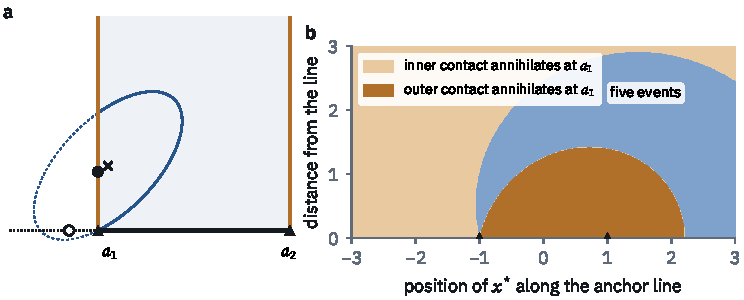
\includegraphics[width=\linewidth]{fig13_unequal.pdf}
\caption{Unequal noise, $\omega_1 = 2\omega_2$ (range 1 noisier, $\eta = 0.6$). (a) Residual coordinates, rotated as in
Figure~\ref{fig:residual}, for $D = 2$ and noise-free point $(-1.5, 0.6)$: the ellipse $\Delta = \Delta(a_1)$ passes through
the corner $a_1$; the weighted foot of the base line (open circle) lies beyond $a_1$, while the foot on the ray beyond
$a_1$ (filled) lies inside its edge. The inner contact and the anchor $a_1$ annihilate. (b) Positions of the noise-free
point (anchors at $\pm1$) at which a contact annihilates at $a_1$, $62\%$ of the area shown; in the blue region all five
events occur.}
\label{fig:unequal}
\end{figure}

\begin{remark}[What carries over]\label{rem:unequal}
Two cavities coexist at some noise level if and only if no foot leaves its edge and
$t_2^2(1 - \eta^2) < t_*^2 + t_1^2 - 2\eta t_* t_1$ and $t_1^2(1 - \eta^2) < t_*^2 + t_2^2 + 2\eta t_* t_2$; at $\eta = 0$ this
is Corollary~\ref{cor:first}(iii). In whitened coordinates $\bar e = W^{1/2}e$ the ellipse is a disc and every wall
distance is divided by $\bar\omega$, so the staircase criterion of Proposition~\ref{prop:criterion} becomes
$\Delta_\alpha < t_{\min}^2/\bar\omega^2$, the disc of radius $R_W = \sqrt2\,t_{\min}/\bar\omega$ lying inside the whitened half-strip.
Theorem~\ref{thm:staircaseW} gives an explicit noise level below which this holds. Whitening also explains Theorem~\ref{thm:unequal}: it maps the right-angled
corners of $F$ to corners of angles $\arccos(-\eta)$ at $a_1$ and $\arccos\eta$ at $a_2$, so the corner of the noisier
range is obtuse, and only at an obtuse corner can the foot of a perpendicular from an interior point land beyond it.
The first event is the nearest boundary point of the whitened half-strip, which for a convex polygon is never a
corner. In high dimension,
$\mathcal E_\sigma = \log\tilde h - \tilde e^\top W\tilde e/2\sigma^2$ is still strictly concave, and Lemma~\ref{lem:cdepth} and
Theorem~\ref{thm:high} hold with $\delta^* = \tilde e^{*\top}W\tilde e^*/2$, $H = -\nabla^2\log\tilde h + W/\sigma^2$ and
$g^2 = (W\tilde e^*)^\top H^{-1}(W\tilde e^*)$.
\end{remark}

\begin{remark}[Other noise laws]\label{rem:noise2}
Let both ranges have noise with density $\propto e^{-V(|\varepsilon|)}$, $V$ convex and strictly increasing. The depth
$V(|e_1|) + V(|e_2|)$ is convex in residual coordinates, so the proof of Proposition~\ref{prop:axis} applies as it stands:
every HPD region is a convex set cut by the walls of $F$, and $m$ is the number of edges it meets minus the number of
corners it contains, with five critical depths, the minima of the depth over the three edges and its values at the two
corners. For exponential-power noise, $V(v) = v^p$, the posterior is an exponential family in $\sigma^{-p}$ and
Theorem~\ref{thm:depth} orders these events in $\sigma$. For Laplace noise ($p = 1$) the regions are $\ell^1$ balls,
whose sides are parallel to the walls, so a wall is met along a whole segment at once. When $t_1, t_2 \le t_*$ that
segment contains both corners: the base contact and both anchors occur at the same depth $2t_*$, and $m$ falls by one
in a single step, a contact that fills a hole. For $x^* = (0.1, 3)$ with anchors at $\pm1$ the region goes two pieces
$\to$ one $\to$ one hole $\to$ one, never passing through the two holes that Gaussian noise produces for the same
triangle.
\end{remark}

%======================================================================
\section{A certified staircase}\label{sec:staircase}

Below some noise level the region has exactly the noise-free shape: two pieces in the plane, a tube in space. By
Proposition~\ref{prop:axis} this regime ends when $\Delta_\alpha(\sigma)$ first reaches $t_{\min}^2$, but
$\Delta_\alpha(\sigma)$ is known only numerically. We give an explicit noise level below which the noise-free topology
is proved. Throughout,
\[ R = \sqrt2\,t_{\min}, \qquad r_{\min} = \min(r_1, r_2), \qquad y = R^2/2\sigma^2 , \]
so $R$ is the distance from the origin to the nearest wall of $F$ and the HPD disc has radius $\sqrt{2\Delta_\alpha}$.

\begin{proposition}[Staircase criterion]\label{prop:criterion}
$\HPD$ has the noise-free topology if and only if $\Delta_\alpha(\sigma) < t_{\min}^2$, that is, if and only if the
HPD disc lies inside $F$. In particular it has the noise-free topology whenever $\Pi_\sigma(|e| \ge R) < \alpha$.
\end{proposition}

\begin{proof}
By Proposition~\ref{prop:axis} the topology is the noise-free one exactly when $m = 0$, i.e.\ when the closed disc of
radius $\sqrt{2\Delta_\alpha}$ misses $\partial F$, i.e.\ when $\sqrt{2\Delta_\alpha} < R$. At equality the disc touches a
wall at one point, $m = 1$, and the topology has already changed. If $\Pi_\sigma(|e| \ge R) < \alpha$ then
$\Pi_\sigma(\Delta < t_{\min}^2) > 1 - \alpha = \Pi_\sigma(\Delta \le \Delta_\alpha)$, so $\Delta_\alpha < t_{\min}^2$.
\end{proof}

The problem is therefore to bound the posterior mass outside the disc $|e| < R$, which requires control of the weight
$J$. The height has a closed form in residual coordinates. Let $\ell_*, \ell_1, \ell_2$ be the distances from $e$ to the
three walls, $s' = (D + w_1 + w_2)/2 = s + (e_1 + e_2)/2$, and $h_0 = 2(st_*t_1t_2)^{1/2}/D$ the height of $T$.

\begin{lemma}[The weight]\label{lem:weight}
\begin{enumerate}[label=(\roman*)]
\item $s' - D = \ell_*/\sqrt2$, $s' - w_1 = \ell_2/\sqrt2$, $s' - w_2 = \ell_1/\sqrt2$, and by Heron's formula
$h^2 = \sqrt2\,s'\ell_*\ell_1\ell_2/D^2$.
\item Let $\Theta(u) = \prod_{c \in \mathcal C}(1 + u/c)$ with $\mathcal C = \{\sqrt2 s, \sqrt2 t_*, \sqrt2 t_1, \sqrt2 t_2\}$. On $F$,
\[ h \le h_0\,\Theta(|e|)^{1/2}, \qquad\text{and}\qquad h \ge h_0\,\Theta(-|e|)^{1/2} \ \text{ when } |e| < R . \]
\item For $d \ge 3$ and $0 < \beta < 1$, with $P(u) = (r_1 + u)(r_2 + u)\,h_0^{d-3}\Theta(u)^{(d-3)/2}$,
\begin{gather*}
J(e) \le P(|e|) \ \text{ on } F, \\
J(e) \ge J_\beta := (r_1 - \beta R)(r_2 - \beta R)\,h_0^{d-3}\Theta(-\beta R)^{(d-3)/2} \ \text{ on } \{|e| \le \beta R\},
\end{gather*}
and $P(u) \le P(R)\,e^{\gamma(u - R)}$ for $u \ge R$, where
$\gamma = \frac{1}{r_1 + R} + \frac{1}{r_2 + R} + \frac{d-3}{2}\sum_{c \in \mathcal C}\frac{1}{c + R}$.
\item For $d = 2$, $J = w_1w_2/h = D/\sin\angle a_1 x a_2 \ge D$ on $F$.
\end{enumerate}
\end{lemma}

\begin{proof}
(i) $s' - D = t_* + (e_1 + e_2)/2 = (e_1 + e_2 + 2t_*)/2 = \ell_*/\sqrt2$, and the other two likewise. Heron gives
$(\tfrac12 Dh)^2 = s'(s' - D)(s' - w_1)(s' - w_2) = s'\ell_*\ell_1\ell_2/2\sqrt2$. (ii) Moving $e$ by $|e|$ from the origin
changes each $\ell_k$ by at most $|e|$ and $s'$ by at most $|e|/\sqrt2$; at the origin $\ell_k = \sqrt2\,t_k$, and
$h_0^2 = \sqrt2\,s\prod_k(\sqrt2\,t_k)/D^2$. Hence $h^2/h_0^2 = (s'/s)\prod_k \ell_k/(\sqrt2\,t_k)$ lies between
$\Theta(-|e|)$ and $\Theta(|e|)$; the lower bound is positive when $|e| < R$ because every $c \in \mathcal C$ is at least $R$.
(iii) $r_i - |e| \le w_i \le r_i + |e|$, and $r_i = t_* + t_i \ge \sqrt2 R > \beta R$. Each factor of $P(u)/P(R)$ has the
form $(c + u)/(c + R) \le e^{(u - R)/(c + R)}$, by concavity of the logarithm. (iv) Twice the area of the triangle is
$Dh = w_1w_2\sin\angle a_1xa_2$.
\end{proof}

\begin{theorem}[Staircase bound]\label{thm:staircase}
For $\sigma \le \sigma_1$ the $1 - \alpha$ HPD region has the noise-free topology (two pieces for $d = 2$, a tube
$\simeq S^{d-2}$ for $d \ge 3$), where:
\begin{enumerate}[label=(\roman*)]
\item for $d = 2$ and $\alpha \le 0.05$,
\[ \sigma_1 = \frac{R}{\sqrt{2L + 2\ln(2L)}}, \qquad L = \ln\frac{2.4\,r_{\min}}{\alpha R}; \]
\item for $d \ge 3$ and any $\beta \in (0,1)$, with $K = P(R)/J_\beta$,
\[ \Lambda(y) = \frac{2y}{2y - \gamma R}\Bigl(1 + \frac{1}{2y - \gamma R}\Bigr)\frac{1}{1 - e^{-\beta^2 y}}, \qquad
   y_0 = \ln\frac{K}{\alpha}, \]
provided $2y_0 > \gamma R$,
\[ \sigma_1 = \frac{R}{\sqrt{2\ln\bigl(K\Lambda(y_0)/\alpha\bigr)}} . \]
\end{enumerate}
\end{theorem}

Explicitly, $K = \frac{(r_1 + R)(r_2 + R)}{(r_1 - \beta R)(r_2 - \beta R)}\bigl[\Theta(R)/\Theta(-\beta R)\bigr]^{(d-3)/2}$, the factors
$h_0$ cancelling; for $d = 3$ the bracket is absent. We use $\beta = 1/\sqrt d$.

\begin{proof}
(ii) By Lemma~\ref{lem:residual}(ii), $\Pi_\sigma(|e| \ge R) = N/Z$, where $N$ and $Z$ are the integrals of
$e^{-|e|^2/2\sigma^2}J$ over $F \cap \{|e| \ge R\}$ and over $F$; since the disc $|e| \le \beta R$ lies inside $F$, $Z$ is at
least the integral over that disc. In polar coordinates, by Lemma~\ref{lem:weight}(iii) and $u^2 \ge R^2 + 2R(u - R)$,
\begin{align*}
N &\le 2\pi P(R)\int_R^\infty u\,e^{\gamma(u - R) - u^2/2\sigma^2}\dd u
   \le 2\pi P(R)e^{-y}\int_0^\infty (R + v)e^{-\lambda v}\dd v\\
  &= 2\pi P(R)e^{-y}R^2\Bigl[\frac{1}{2y - \gamma R} + \frac{1}{(2y - \gamma R)^2}\Bigr],
\end{align*}
with $\lambda = (2y - \gamma R)/R > 0$, and $Z \ge J_\beta\cdot 2\pi\sigma^2(1 - e^{-\beta^2 y})$ with $\sigma^2 = R^2/2y$.
Dividing, $\Pi_\sigma(|e| \ge R) < K e^{-y}\Lambda(y)$, strictly because $Z$ also has mass outside $|e| \le \beta R$.
Each factor of $\Lambda$ is at least $1$ and decreasing in $y$. Put $y_1 = \ln(K\Lambda(y_0)/\alpha) \ge y_0$; for
$y \ge y_1$, $Ke^{-y}\Lambda(y) \le Ke^{-y_1}\Lambda(y_0) = \alpha$. Since $\sigma \le \sigma_1$ is exactly $y \ge y_1$,
Proposition~\ref{prop:criterion} applies.

(i) For $d = 2$ the weight $J = D/\sin\angle a_1xa_2$ is unbounded at the walls, so we bound the numerator in the plane
instead. Use polar coordinates about $a_i$ with $r_i = r_{\min}$, $\dd x = w_i\dd w_i\dd\phi$, and fix $e_i$. On
$\{S \ge R^2\}$ the integrand $e^{-S/2\sigma^2}$ is at most $e^{-y}$, and it is at most $e^{-e_i^2/2\sigma^2}$ everywhere; so the
angular integral is at most $2\pi e^{-y}$ when $|e_i| \le R$ and at most $2\pi e^{-e_i^2/2\sigma^2}$ when $|e_i| > R$. With $r_i > R$ and the Mills ratio
$\int_R^\infty e^{-v^2/2\sigma^2}\dd v \le (\sigma^2/R)e^{-y}$,
\begin{align*}
\int_{S \ge R^2} e^{-S/2\sigma^2}\dd x
 &\le 2\pi\Bigl[e^{-y}\!\int_{-R}^{R}(r_i + e)\dd e + \!\int_{|e| > R,\, e > -r_i}\!(r_i + e)e^{-e^2/2\sigma^2}\dd e\Bigr]\\
 &\le 2\pi e^{-y}\Bigl[2Rr_i + \sigma^2\Bigl(\frac{2r_i}{R} + 1\Bigr)\Bigr].
\end{align*}
By Lemma~\ref{lem:weight}(iv), applied on both half-planes,
$\int_{\R^2} e^{-S/2\sigma^2}\dd x \ge 2\int_{|e| < R} e^{-|e|^2/2\sigma^2}\dd e = 4\pi\sigma^2(1 - e^{-y})$. With
$\mu = r_{\min}/R \ge \sqrt2$ this gives
\[ \Pi_\sigma(|e| \ge R) \le y e^{-y} G(y), \qquad G(y) = \frac{2\mu + (\mu + \frac12)/y}{1 - e^{-y}} , \]
and $G$ is decreasing. For $\alpha \le 0.05$, $L \ge \ln(48\sqrt2) > 4.2$, and $G(4.2) < 2.36\,\mu$ because
$\mu \ge \sqrt2$. So for $y \ge L$, $\Pi_\sigma(|e| \ge R) < 2.4\,\mu\,y e^{-y}$, which is at most $\alpha$ as soon as
$y - \ln y \ge L$. This holds for $y \ge L + \ln(2L)$, since $y - \ln y$ is increasing for $y > 1$ and $L > \ln(2L)$ for
all $L > 0$; and $y \ge L + \ln(2L)$ is exactly $\sigma \le \sigma_1$.
\end{proof}

Since $\sigma_1$ depends only on the observed $(D, r_1, r_2)$, $d$ and $\alpha$, Theorem~\ref{thm:staircase} is a certificate
computable from the data: whenever the known noise level is at most $\sigma_1$, the credible region provably has the
noise-free shape, and no summary with a convex credible region can describe it.

If the posterior were exactly an isotropic Gaussian on the plane, the staircase would end at
$\sigma = R/\sqrt{2\ln(1/\alpha)}$. For $d \ge 3$ the proved bound has the same form with $1/\alpha$ replaced by
$K\Lambda(y_0)/\alpha$: the whole price of rigour is one geometric constant.

\paragraph{Unequal noise} With noise $\sigma \omega_i$ on range $i$ (\S\ref{sec:unequal}), the same method works in whitened
coordinates $\bar e = W^{1/2}e$, where the HPD region is the disc $|\bar e|^2 \le 2\Delta_\alpha$ and the
noise-free topology holds if and only if that disc has radius below $R_W = R/\bar\omega$ (Remark~\ref{rem:unequal}). Put
$R_i = (\omega_i/\bar\omega)R$ and, now, $y = R_W^2/2\sigma^2$.

\begin{theorem}[Staircase bound, unequal noise]\label{thm:staircaseW}
For $\sigma \le \sigma_1$ the $1 - \alpha$ HPD region has the noise-free topology, where:
\begin{enumerate}[label=(\roman*)]
\item for $d = 2$ and $\alpha \le 1/2$, with $i$ either anchor, $j$ the other, $\mu_i = r_i/(\omega_jR_W)$ and
$G_i(y) = \bigl(2\mu_i + (\mu_i + \omega_i/2\omega_j)/y\bigr)/(1 - e^{-y})$,
\[ \sigma_1 = \frac{R_W}{\sqrt{2L + 2\ln(2L)}}, \qquad L = \ln\frac{G_i\bigl(\ln(2\mu_i/\alpha)\bigr)}{\alpha}; \]
\item for $d \ge 3$ and any $\beta \in (0,1)$, with
\[ K_W = \frac{(r_1 + R_1)(r_2 + R_2)}{(r_1 - \beta R_1)(r_2 - \beta R_2)}\Bigl[\frac{\Theta(R)}{\Theta(-\beta R)}\Bigr]^{\frac{d-3}{2}}, \quad
   \gamma_W = \sum_{i=1}^2\frac{R_i}{r_i + R_i} + \frac{d-3}{2}\sum_{c \in \mathcal C}\frac{R}{c + R}, \]
$\Lambda_W(y) = \frac{2y}{2y - \gamma_W}\bigl(1 + \frac{1}{2y - \gamma_W}\bigr)\frac{1}{1 - e^{-\beta^2 y}}$ and
$y_0 = \ln(K_W/\alpha)$, provided $2y_0 > \gamma_W$,
\[ \sigma_1 = \frac{R_W}{\sqrt{2\ln\bigl(K_W\Lambda_W(y_0)/\alpha\bigr)}} . \]
\end{enumerate}
For $\omega_1 = \omega_2$, (ii) is Theorem~\ref{thm:staircase}(ii), and (i), centred at the anchor of the shorter range, is at
least the value of Theorem~\ref{thm:staircase}(i), since then $G_i(\ln(2\mu_i/\alpha)) < 2.38\,\mu_i$ for $\alpha \le 0.05$.
\end{theorem}

\begin{proof}
Write $e_i = \omega_i\bar e_i$. The wall normals are $n = (1, \pm1)/\sqrt2$, and by Cauchy--Schwarz
$|n\cdot e| = |\omega_1\bar e_1 \pm \omega_2\bar e_2|/\sqrt2 \le \bar\omega|\bar e|$. So, with $u = \bar\omega|\bar e|$, the
wall distances lie within $u$ of $\sqrt2\,t_k$, $s'$ lies within $u/\sqrt2$ of $s$, and $|w_i - r_i| \le \omega_i|\bar e|$:
Lemma~\ref{lem:weight} holds with $|e|$ replaced by $u$ in the bounds on $h$ and by $\omega_i|\bar e|$ in those on $w_i$, and
at $|\bar e| = R_W$, $u = R$. Since $\omega_i < \sqrt2\,\bar\omega$, $R_i < \sqrt2 R = 2t_{\min} \le r_i$, so every lower bound
stays positive for $\beta < 1$.

(ii) The proof of Theorem~\ref{thm:staircase}(ii) applies in $\bar e$, whose Jacobian is constant: each factor of the
bound $P_W(|\bar e|)$ on $J$ is of the form $c + b|\bar e|$, so
$P_W(\varrho) \le P_W(R_W)e^{\gamma_W(\varrho - R_W)/R_W}$ for $\varrho \ge R_W$, and the integrals are those of
Theorem~\ref{thm:staircase} with $R$ replaced by $R_W$ and $\gamma R$ by $\gamma_W$.

(i) As in Theorem~\ref{thm:staircase}(i), in polar coordinates about $a_i$: on $\{|\bar e| \ge R_W\}$ the density is at
most $e^{-y}$, and everywhere at most $e^{-e_i^2/2\sigma^2\omega_i^2}$, so with the Mills ratio
\[ \int_{|\bar e| \ge R_W} e^{-|\bar e|^2/2\sigma^2}\dd x \le 2\pi \omega_i e^{-y}\Bigl[2R_Wr_i + \sigma^2\Bigl(\frac{2r_i}{R_W} + \omega_i\Bigr)\Bigr], \]
while the total mass is at least $2\omega_1\omega_2\cdot 2\pi\sigma^2(1 - e^{-y})$, by Lemma~\ref{lem:weight}(iv) and
$\dd e = \omega_1\omega_2\dd\bar e$. Dividing, $\Pi_\sigma(|\bar e| \ge R_W) \le ye^{-y}G_i(y)$. Now $G_i$ is decreasing,
$G_i \ge 2\mu_i$, and $\mu_i \ge \sqrt2\,\bar\omega/\omega_j > 1$, so $L \ge \ln(2\mu_i/\alpha) > \ln 4 > 1$ for $\alpha \le 1/2$.
For $y \ge L + \ln(2L)$ we get $ye^{-y}G_i(y) \le \alpha\,ye^{L - y} \le \alpha$, since $y - \ln y$ is increasing for
$y > 1$ and $L \ge \ln(2L)$.
\end{proof}

The certificate depends on the noise levels only through the ratios $\omega_i/\bar\omega < \sqrt2$, and it is as sharp as with
equal noise. For the four geometries $x^* = (0.2, 1.1)$, $(0, 1)$, $(0.3, 1.4)$, $(0, 3.7)$, noise ratios
$\omega_1 : \omega_2 = 1 : 1$, $2 : 1$, $1 : 4$ and $d = 2, 3, 4$, the proved $\sigma_1$ is $0.64$--$0.81$ of the true first
transition, and for a fixed geometry and dimension the ratio changes by at most $0.03$ with the noise ratio
(Supplement~\ref{app:comp}).

\paragraph{How sharp it is} Table~\ref{tab:sharp} compares $\sigma_1$ with the exact first transition, computed by
quadrature in residual coordinates (Supplement~\ref{app:comp}). The bound is sharpest in $d = 3$, at $71$--$87\%$ of the exact value, where $J = w_1w_2$ involves no
height. It weakens in two places, for two different reasons. In higher dimension ($48$--$70\%$ at $d = 10$) the factor
$h^{d-3}$ must be bounded above outside the disc and below inside the smaller disc $|e| \le \beta R$; each bound loses
a constant factor and both are raised to the power $(d-3)/2$, so $\ln K$ grows linearly in $d$ while the true threshold
falls slowly. In the plane ($58$--$70\%$), bounding a whole angular integral by $2\pi$ to avoid the singular weight costs
a factor of order $r_{\min}/R$, which is largest for flat triangles, where $t_{\min}$ is small compared with the ranges.
In $d \ge 3$ the opposite holds and flat triangles are where the bound is best. At $\sigma = \sigma_1$ the true mass
outside the disc is between $10^{-4}$ and $2\cdot10^{-2}$ for $d \le 4$ (and as small as $10^{-7}$ at $d = 10$), against
the allowed $5\cdot10^{-2}$: the slack sits in the constant, not in the method.

\begin{table}[t]\centering\small
\caption{Proved over exact first threshold, $\sigma_1/\sigma_1^{\mathrm{exact}}$, at $\alpha = 0.05$, symmetric geometry
with crossing angle $\theta$ (anchors at $\pm1$, $\beta = 1/\sqrt d$). For the asymmetric example $D = 2$,
$x^* = (0.2, 1.1)$: $0.67$ ($d = 2$) and $0.78$ ($d = 3$).}\label{tab:sharp}
\begin{tabular}{rc@{\qquad}ccccc}\toprule
$\theta$ & $\sigma_1^{\mathrm{exact}}$ ($d = 2$) & $d = 2$ & $d = 3$ & $d = 4$ & $d = 6$ & $d = 10$\\\midrule
$30^\circ$ & 0.560 & 0.67 & 0.77 & 0.64 & 0.54 & 0.48\\
$60^\circ$ & 0.570 & 0.70 & 0.71 & 0.62 & 0.55 & 0.51\\
$90^\circ$ & 0.237 & 0.66 & 0.79 & 0.71 & 0.64 & 0.59\\
$120^\circ$ & 0.0876 & 0.63 & 0.84 & 0.76 & 0.70 & 0.66\\
$150^\circ$ & 0.0198 & 0.58 & 0.87 & 0.80 & 0.74 & 0.70\\\bottomrule
\end{tabular}
\end{table}

%======================================================================
\section{High dimension}\label{sec:high}

How do the transitions of \S\ref{sec:two} behave as $d$ grows? The natural scaling keeps the triangle's shape and
lets its size grow with the typical distance in $\R^d$: fix a non-degenerate triangle $(\tilde D, \tilde r_1, \tilde r_2)$
and put $D = \sqrt d\,\tilde D$, $r_i = \sqrt d\,\tilde r_i$, with $\sigma$ fixed. A tilde denotes a length divided by
$\sqrt d$; so $\tilde e = e/\sqrt d$ lies in the scaled half-strip $\tilde F = F/\sqrt d$, and $\tilde t_*, \tilde t_1, \tilde t_2$
are the scaled tangent lengths. The answer is that the posterior concentrates at a single point, which residual
coordinates identify exactly; the mechanism is the Laplace method \citep{wong1989}, made available by a concavity that
the residual coordinates reveal. The proofs of this section are in Supplement~\ref{app:high}.

\begin{lemma}[The concentration point]\label{lem:conc}
In scaled residual coordinates the posterior density of $\tilde e$ is proportional to
\[ \exp\bigl((d - 3)\,\mathcal E_\sigma(\tilde e)\bigr)\,\tilde w_1\tilde w_2\,e^{-3|\tilde e|^2/2\sigma^2}, \qquad
   \mathcal E_\sigma(\tilde e) = \log\tilde h(\tilde e) - \frac{|\tilde e|^2}{2\sigma^2}, \]
on $\tilde F$. The function $\mathcal E_\sigma$ is strictly concave, tends to $-\infty$ at $\partial\tilde F$ and at infinity, and
has a unique maximiser $\tilde e^*(\sigma)$, which lies in the interior of $\tilde F$ and is never $0$. For a symmetric
triangle, $\tilde e^* = (u, u)$ with $u > 0$.
\end{lemma}

For a symmetric triangle the posterior therefore overshoots both ranges. The factor $\tilde h^{d}$ is the volume of the
$(d-2)$-sphere of points with the given residuals, and in high dimension this volume outweighs the likelihood, exactly as
the radial mode of one range sits beyond $r$. For an asymmetric triangle the push is not along the diagonal: for small
$\sigma$, $\tilde e^* = \sigma^2\nabla\log\tilde h(0) + O(\sigma^4)$, so range $i$ is overshot exactly when
$1/\tilde s + 1/\tilde t_* + 1/\tilde t_i > 1/\tilde t_j$, and a very short tangent length $\tilde t_j$ makes the other range
undershot.

\begin{lemma}[The concentration depth]\label{lem:cdepth}
Let $\delta^*(\sigma) = |\tilde e^*(\sigma)|^2/2$ and $H = -\nabla^2\mathcal E_\sigma(\tilde e^*)$, so $H \succeq I/\sigma^2$. Then
$\tilde e^*$ is $C^1$ in $\sigma$, with $\dd\tilde e^*/\dd\sigma = (2/\sigma^3)H^{-1}\tilde e^*$, and $\delta^*$ increases strictly
from $0$ to $\infty$, with
\[ \delta^{*\prime}(\sigma) = \frac{2\,g(\sigma)^2}{\sigma^3}, \qquad g(\sigma)^2 = \tilde e^{*\top}H^{-1}\tilde e^* . \]
\end{lemma}

The same $g$ reappears below as a standard deviation, for the reason behind Theorem~\ref{thm:depth}: in
$\tau = 1/\sigma^2$ the posterior is an exponential family with statistic $-\Delta$, so $\dd E[\Delta]/\dd\tau = -\mathrm{Var}(\Delta)$,
and to leading order $E[\Delta] = d\,\delta^*$ and $\mathrm{Var}(\Delta) = d\,g^2$.

\begin{theorem}[High dimension]\label{thm:high}
Uniformly for $\sigma$ in compact subsets of $(0, \infty)$ and triangle shapes in compact sets of non-degenerate
triangles,
\[ \Delta_\alpha(\sigma) = d\,\delta^*(\sigma) + z\sqrt d\,g(\sigma) + o(\sqrt d). \]
Consequently a transition of scaled depth $\tilde\Delta_c$ (one of $\tilde t_*^2, \tilde t_1^2, \tilde t_2^2, \tilde t_*^2 + \tilde t_i^2$)
occurs at
\[ \sigma_c(d) = \sigma_{c,\infty} - \frac{z\,\sigma_{c,\infty}^3}{2\,g(\sigma_{c,\infty})\sqrt d} + o(d^{-1/2}),
   \qquad \delta^*(\sigma_{c,\infty}) = \tilde\Delta_c . \]
\end{theorem}

The limit $\sigma_{c,\infty}$ does not depend on $\alpha$: at scale $d$ the posterior is pinned to one point, and the
credibility level only decides where in the $O(\sqrt d)$ cloud around it the cut falls. This is why the approach to the
limit is slow, of order $1/\sqrt d$.

\begin{corollary}[Closed forms]\label{cor:closed}
For the symmetric triangle with $\tilde r_1 = \tilde r_2 = 1$ and $\tilde D = 2\zeta$, $\zeta = \sin(\theta/2)$, the first transition
occurs at
\[ \sigma_1(d) = \sqrt{\frac{8(1-\zeta)^2}{2-\zeta}} - \frac{2z\,(1-\zeta)\sqrt{\zeta^2 - 4\zeta + 6}}{(2-\zeta)^{3/2}\sqrt d} + o(d^{-1/2})
   \qquad (\theta \ge 60^\circ), \]
and, for $\theta < 60^\circ$, at
\[ \sigma_1(d) = \sqrt{\frac{2\zeta(1+2\zeta)}{1+\zeta}} - z\sqrt{\frac{(1+2\zeta)(2\zeta^3 + 4\zeta^2 + 4\zeta + 1)}{2(1+\zeta)^3}}\,\frac{1}{\sqrt d} + o(d^{-1/2}).
\]
The two formulas agree at $\theta = 60^\circ$, where all three contacts coincide. At $\theta = 90^\circ$ and $\alpha = 0.05$,
$\sigma_1(d) = 0.7286 - 1.256/\sqrt d + o(d^{-1/2})$. For one range the same argument gives
$\sigma = \sqrt2 - 2z\sqrt{3/8}/\sqrt d + o(d^{-1/2})$, which is $r/\kappa_d$ with $r = \sqrt d$ by Theorem~\ref{thm:main}(c).
\end{corollary}

Figure~\ref{fig:high} compares these formulas with the first transition computed exactly at finite $d$
(Supplement~\ref{app:comp}). Extrapolating the values at $d = 160$, $640$ and $2560$ in powers of $d^{-1/2}$ lands within
$0.02\%$ of $\sigma_{1,\infty}$ at every angle shown, and the two-term formula of Corollary~\ref{cor:closed} is within
$1.8\%$, $0.43\%$ and $0.11\%$ of the exact values at these dimensions: the error falls by a factor of about four for
each fourfold increase in $d$, consistent with an $O(1/d)$ remainder. For a triangle of fixed size the scaling says that the thresholds eventually fall
like $r\,\sigma_{c,\infty}(\theta)/\sqrt d$.

\begin{figure}[t]\centering
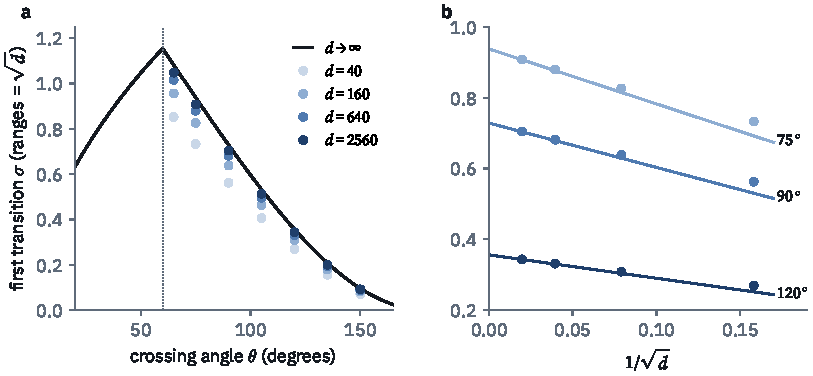
\includegraphics[width=\linewidth]{fig11_high_dim.pdf}
\caption{Two ranges in high dimension, symmetric geometry, ranges $= \sqrt d$, $\alpha = 0.05$. (a) The first transition
computed exactly at $d = 40$ to $2560$ (dots) against the limit $\sigma_{1,\infty}(\theta)$ of Corollary~\ref{cor:closed} (curve; the
outer contacts come first left of $60^\circ$, the inner contact right of it). (b) The same values against $1/\sqrt d$ at
$75^\circ$, $90^\circ$ and $120^\circ$, with the two-term formula $\sigma_{1,\infty} - zC/\sqrt d$ (lines).}
\label{fig:high}
\end{figure}

%======================================================================
\section{Random anchors}\label{sec:random}

\begin{figure}[t]\centering
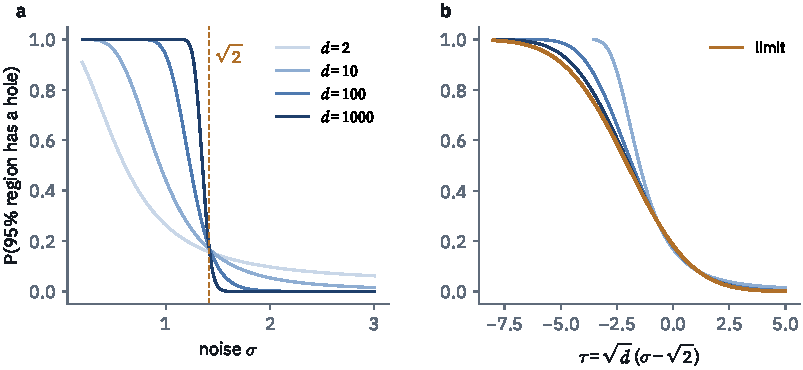
\includegraphics[width=\linewidth]{fig9_sqrt2.pdf}
\caption{(a) The probability of a hole for a random anchor, $P_d(\sigma)$, for $d = 2, 10, 100, 1000$: the curves
sharpen into a step at $\sqrt2$. (b) The same probability against $\tau = \sqrt d(\sigma - \sqrt2)$ for
$d = 10, 100, 1000$, converging to the limit of Theorem~\ref{thm:sqrt2}(iii).}
\label{fig:sqrt2}
\end{figure}

\paragraph{One range} Let the anchor be random, $a \sim N(0, I_d)$, with independent noise $Z \sim N(0,1)$; the truth is
$x^* = 0$ and $r = \|a\| + \sigma Z$. The posterior treats the realised anchor as known, so the randomness enters only
through which posterior we obtain. Let $P_d(\sigma)$ be the probability that its $\HPD$ has a hole, and
$\delta_0 = z\sqrt{3/8}$.

\begin{theorem}\label{thm:sqrt2}
\begin{enumerate}[label=(\roman*)]
\item $P_d(\sigma) = \Pr\bigl(\|a\| + \sigma Z > \kappa_d(\alpha)\sigma\bigr)$, where $\|a\| \sim \chi_d$ is independent of $Z$.
\item $P_d(\sigma) \to 1$ if $\sigma < \sqrt2$ and $P_d(\sigma) \to 0$ if $\sigma > \sqrt2$, as $d \to \infty$.
\item For $\sigma_d = \sqrt2 + \tau/\sqrt d$,
$\displaystyle\lim_{d \to \infty} P_d(\sigma_d) = 1 - \Phi\Bigl(\frac{\sqrt2\,\delta_0 + \tau/\sqrt2}{\sqrt{5/2}}\Bigr)$.
\end{enumerate}
\end{theorem}

\begin{proof}
(i) is Theorem~\ref{thm:main}(a) conditionally on $(a, r)$; when $r \le 0$ there is no hole, consistently with
$\kappa_d > 0$. (ii) $\|a\|^2$ has mean $d$ and variance $2d$, so $\|a\|/\sqrt d \to 1$ in probability \citep[\S3.1]{vershynin2018}, and
$\kappa_d/\sqrt d \to 1/\sqrt2$; hence $(\|a\| + \sigma Z - \kappa_d\sigma)/\sqrt d \to 1 - \sigma/\sqrt2$ in probability.
(iii) By the central limit theorem and Slutsky's lemma, $\|a\| - \sqrt d = (\|a\|^2 - d)/(\|a\| + \sqrt d) \to N(0, 1/2)$.
By Theorem~\ref{thm:main}(c), $\kappa_d\sigma_d = \sqrt d + \tau/\sqrt2 + \sqrt2\,\delta_0 + o(1)$, so
$\|a\| + \sigma_dZ - \kappa_d\sigma_d \to N(0, 1/2 + 2) - (\sqrt2\,\delta_0 + \tau/\sqrt2)$ in law.
\end{proof}

At $\alpha = 0.05$ and $\tau = 0$ the limit is $1 - \Phi(1.42448/1.58114) = 0.1838$; the exact values are $0.1783$ at
$d = 100$ and $0.1832$ at $d = 10^4$. The limit at $\sigma = \sqrt2$ is not $1/2$: the offset $\delta_0$ moves the 50\%
point to $\sigma_{1/2}(d) = \sqrt2 - 2\delta_0/\sqrt d + o(1/\sqrt d)$, which is $2.015/\sqrt d$ to the left of $\sqrt2$.
The value $\sqrt2$ itself is where the typical anchor distance $\sqrt d$ equals the threshold range
$\kappa_d\sigma \approx \sigma\sqrt{d/2}$. The window is $1/\sqrt d$ because the margin
$\|a\| + \sigma Z - \kappa_d\sigma$ has mean about $\sqrt d(1 - \sigma/\sqrt2)$ but fluctuations of order one.


\paragraph{Two ranges} Now let $a_1, a_2 \sim N(0, I_d)$ be independent, $x^* = 0$, and $r_i = \|a_i\| + \sigma\varepsilon_i$.
The scaled triangle converges to the right isosceles triangle $(\tilde r_1, \tilde r_2, \tilde D) = (1, 1, \sqrt2)$, and
Theorem~\ref{thm:high} turns this into a sequence of sharp transitions.

\begin{theorem}\label{thm:random2}
Fix $\alpha \in (0,1)$. As $d \to \infty$, with probability tending to one the $1-\alpha$ HPD region
\begin{enumerate}[label=(\roman*)]
\item has the noise-free topology, a tube $\simeq S^{d-2}$, if $\sigma < 0.7286 = \sigma_{1,\infty}(90^\circ)$;
\item is contractible if $0.7286 < \sigma < \sqrt2$ or $\sigma > 1.5062$;
\item has exactly two cavities, $\beta_{d-1} = 2$, if $\sqrt2 < \sigma < 1.5062$.
\end{enumerate}
\end{theorem}

\begin{proof}
$\|a_i\|/\sqrt d \to 1$ and $\|a_1 - a_2\|/\sqrt d \to \sqrt2$ in probability, and $\sigma\varepsilon_i/\sqrt d \to 0$, so the
observed scaled triangle converges in probability to $T_0 = (1, 1, \sqrt2)$, which is non-degenerate; with probability
tending to one it lies in a compact neighbourhood of $T_0$ of non-degenerate triangles, which is all that
\S\ref{sec:two} requires. The posterior is a function of the observed triangle, so by
Theorem~\ref{thm:high}, uniformly on that neighbourhood, $\Delta_\alpha/d = \delta^*(\sigma; \tilde T) + O(d^{-1/2})$, and by
continuity $\Delta_\alpha/d \to \delta^*(\sigma; T_0)$ in probability, as do the scaled depths of the five transitions. At
$T_0$, $\zeta = 1/\sqrt2$, $\theta = 90^\circ$, and these depths are $\tilde t_*^2 = (1 - 1/\sqrt2)^2$, $\tilde t_1^2 = \tilde t_2^2 = 1/2$
and $\tilde t_*^2 + \tilde t_i^2 = 2 - \sqrt2$; by Corollary~\ref{cor:closed} and its proof they are reached at
$\sigma = 0.7286$, at $\sigma^2 = 2\zeta(1 + 2\zeta)/(1 + \zeta) = 2$, and at $\sigma = 1.5062$. Since $\delta^*$ is strictly increasing,
$m(\Delta_\alpha)$ equals $0$, $1$, $3$, $1$ on the four intervals with probability tending to one (the two outer contacts,
and the two anchors, are crossed in the same interval), and Proposition~\ref{prop:axis} gives the topology.
\end{proof}

So for random anchors in high dimension, more noise first merges the flip pair, then hollows the region out twice,
then fills it: the backwards staircase of \S\ref{sec:two} survives the randomness, at explicit noise levels. Each
transition has a window of width of order $1/\sqrt d$, because the triangle fluctuates by $O(d^{-1/2})$, the same order
as the correction in Theorem~\ref{thm:high}.

When there are as many ranges as dimensions, the noise-free set is a mirror pair and, by Theorem~\ref{thm:nranges},
the region is two pieces exactly while it misses the anchor hyperplane. We expect this to fail only when the truth is
within about $\sqrt\sigma$ of the hyperplane, since moving a distance $h$ off the hyperplane changes every range by
$O(h^2)$. In the plane this is a theorem, up to a logarithm.

\begin{theorem}[A square-root law for flip ambiguity]\label{thm:sqrtlaw}
Let $a_1, a_2 \sim N(0, I_2)$ be independent, $x^* = 0$, $r_i = \|a_i\| + \sigma\varepsilon_i$, and $\alpha \le 1/2$. There are
constants $0 < c \le C$, depending on $\alpha$, such that for small $\sigma$
\[ c\sqrt\sigma \le 1 - \Pr(\text{the HPD region is exactly two pieces}) \le C\sqrt\sigma\,(\log 1/\sigma)^{1/4} . \]
\end{theorem}

The proof is in Appendix~\ref{app:sqrt}. It rests on one observation: $a_1 - a_2$ and $(a_1 + a_2)/2$ are independent, so the
distance $h_0$ from the truth to the anchor line is distributed as $|N(0, 1/2)|$, independently of
the anchor separation and of where the foot of the perpendicular falls. The smallest tangent length of the triangle is of
order $h_0^2$. Theorem~\ref{thm:staircaseW}(i) certifies two pieces once it exceeds $2\sigma(\log 1/\sigma)^{1/2}$, which
costs the logarithm, and when it is below a multiple of $\sigma$ the data are inconsistent with probability bounded
below.

\begin{conjecture}\label{conj:sqrt}
The logarithm in Theorem~\ref{thm:sqrtlaw} can be removed; and for $d \ge 3$, with $d$ anchors
$a_1, \dots, a_d \sim N(0, I_d)$, $1 - \Pr(\text{two pieces})$ is again of exact order $\sqrt\sigma$.
\end{conjecture}

In the plane the event can be evaluated exactly: the region is two pieces if and only if the observed ranges satisfy the
strict triangle inequality (Lemma~\ref{rem:inconsistent}) and $\Delta_\alpha(\sigma) < t_{\min}^2$
(Proposition~\ref{prop:criterion}), which we evaluate by quadrature (Supplement~\ref{app:comp}), or skip whenever
$\sigma \le \sigma_1$ of Theorem~\ref{thm:staircase}(i) already certifies two pieces. With $4000$ trials at each of seven
noise levels from $0.004$ to $0.08$, the failure probability rises from $0.119$ to $0.554$, and a weighted least-squares
fit of $\log\Pr(\text{fail})$ on $\log\sigma$ gives exponent $0.516$, with $95\%$ bootstrap interval $[0.497, 0.535]$. A law
$\sqrt\sigma\,(\log 1/\sigma)^{1/4}$ would have fitted exponent about $0.43$ over this range, which the interval excludes:
this is the evidence for the first half of the conjecture. Inconsistent data account for a little over a
quarter of the failures and scale with exponent $0.50$. For $d \ge 3$, Theorem~\ref{thm:nranges} still decides the event
exactly, but evaluating it needs a $d$-dimensional integral, which we have not carried out at scale. The decomposition of
Appendix~\ref{app:sqrt} does carry over: in $d = 3$ the centroid of the anchors is independent of their differences, so
the distance from the truth to the anchor plane is distributed as $|N(0, 1/3)|$, independently of the anchor triangle.
What is missing for an upper bound is a certificate for three ranges.

%======================================================================
\section{Discussion}\label{sec:discussion}

\paragraph{For practice} Above $\kappa_d$, and inside the staircase regime of two ranges, Gaussian summaries are wrong
in kind. Every Gaussian summary has a convex credible region, whether it matches the posterior's mean and covariance (a
``mean $\pm$ covariance'' report) or its curvature at a mode (a Laplace approximation, or an extended Kalman filter
linearised there), and the posterior mean can sit in a region the posterior excludes. For one range in the plane this
happens as soon as the range exceeds about twice the noise. For two ranges,
Theorem~\ref{thm:staircase} certifies the flip ambiguity from the triangle alone: if $\sigma \le \sigma_1$ the 95\%
region is two separate pieces in the plane, and a tube around the anchor line in space, and any unimodal summary is
wrong.

\paragraph{What it costs} Table~\ref{tab:coverage} measures this by frequentist coverage, for the asymmetric example of
\S\ref{sec:two} in the plane, at six noise levels chosen so that the noise-free data visit all six phases. For each level
we draw $2000$ data sets and compute four $95\%$ regions under the flat prior: the HPD region; the Laplace ellipse at a
posterior mode, choosing one of the two mirror modes at random, since they have equal height; the HPD region of the
equal-weight mixture of the Laplace Gaussians at both mirror modes, which is what a practitioner aware of the flip would
report; and the ellipse of the Gaussian with the posterior mean and covariance. The HPD region covers the true point in
$93.6$--$97.6\%$ of data sets; flat-prior HPD regions carry no exact frequentist guarantee, so this is an empirical
finding, not a theorem. A single Laplace ellipse covers it in about half of the data sets, $46$--$66\%$, as the mirror
symmetry predicts. The mixture repairs this in the two-piece phase, covering $95.4\%$ with about the same area as the
HPD region, but it fails once the region is no longer a union of ellipses: from the first ring on ($\sigma \ge 0.56$) it
covers only $93.0\%$, $90.1\%$, $88.2\%$ and $84.0\%$, against $94.4$--$97.6\%$ for the HPD region, although its
median area is $12$--$31\%$ larger than that of the
HPD region. The moment-matched ellipse covers, but only by being large: at $\sigma = 0.15$ its median area is $3.7$ times
that of the HPD region, and its centre, the posterior mean, lies outside the HPD region in $99\%$ of data sets.

\begin{table}[t]\centering\footnotesize
\caption{Coverage of the true point and median area of four $95\%$ regions: two ranges in the plane, $D = 2$,
$x^* = (0.2, 1.1)$, $2000$ data sets per noise level (Monte Carlo standard error of a coverage between $0.005$ and
$0.011$). Laplace: the ellipse at one posterior mode. Mixture: the HPD region of the equal-weight mixture of the Laplace
Gaussians at the two mirror modes. Moments: the ellipse of the Gaussian with the posterior mean and covariance. Phase:
the topology of the HPD region for the noise-free data. Last column: how often the posterior mean lies in the HPD
region.}
\label{tab:coverage}
\setlength{\tabcolsep}{3.2pt}
\begin{tabular}{rl@{\quad}cccc@{\quad}cccc@{\quad}c}\toprule
& & \multicolumn{4}{c}{coverage} & \multicolumn{4}{c}{median area} & mean\\
$\sigma$ & phase & HPD & Laplace & mixture & moments & HPD & Laplace & mixture & moments & in HPD\\\midrule
0.15 & two pieces & 0.953 & 0.459 & 0.954 & 0.972 & 0.88 & 0.43 & 0.85 & 3.27 & 0.010\\
0.40 & one piece & 0.936 & 0.514 & 0.946 & 0.947 & 6.24 & 3.14 & 6.10 & 9.01 & 0.720\\
0.56 & ring & 0.944 & 0.555 & 0.930 & 0.951 & 9.99 & 6.33 & 11.14 & 12.52 & 0.873\\
0.66 & one piece & 0.948 & 0.591 & 0.901 & 0.962 & 12.51 & 8.94 & 14.45 & 15.14 & 0.904\\
0.75 & ring & 0.958 & 0.607 & 0.882 & 0.969 & 14.62 & 11.69 & 18.10 & 17.14 & 0.931\\
1.00 & one piece & 0.976 & 0.661 & 0.840 & 0.991 & 21.68 & 21.08 & 28.35 & 24.30 & 0.956\\\bottomrule
\end{tabular}
\end{table}

\paragraph{Limitations} We assume a flat prior, Gaussian noise (or the class of Theorem~\ref{thm:noise} for one
range, and Remark~\ref{rem:noise2} for two), noise levels known up to a common factor, and HPD regions; other credible regions can have a different topology. An informative
prior breaks the rotational symmetry the proofs use, and we expect the thresholds to move but not to disappear. With
three or more ranges in the plane, critical points need not lie on any line (\S\ref{sec:three}).

\paragraph{Code} The software that computes every number, table and figure (Supplement~\ref{app:comp}) is available at
\url{https://github.com/mmehta4/posterior-topology}, with one script per table and figure, and archived at
\href{https://doi.org/10.5281/zenodo.23336821}{doi:10.5281/zenodo.23336821}.

\paragraph{Use of AI tools} Claude (Anthropic) assisted with the software and manuscript preparation.



\bibliographystyle{plainnat}
\bibliography{refs}

%======================================================================
\appendix
\section{Proof of Theorem~\ref{thm:sqrtlaw}}\label{app:sqrt}

Throughout, $C$ and $c$ denote positive constants that depend only on $\alpha$, and \emph{fail} is the event that the
region is not exactly two pieces.

\paragraph{Decomposition} Put $a_- = a_1 - a_2 \sim N(0, 2I)$ and $a_+ = (a_1 + a_2)/2 \sim N(0, I/2)$, which are independent.
Let $D = |a_-|$, let $\vartheta$ be a unit vector orthogonal to $a_-$, and put $\xi_0 = a_+\cdot a_-/D$ and
$h_0 = |a_+\cdot\vartheta|$. Given $a_-$, $a_+\cdot a_-/D$ and $a_+\cdot\vartheta$ are independent $N(0, 1/2)$ variables, so
$h_0 \sim |N(0, 1/2)|$, with density at most $2/\sqrt\pi$, and $D$, $\xi_0$, $h_0$ are independent. The anchor line is
$\{a_+ + \lambda a_-\}$, so $h_0$ is the distance from $x^* = 0$ to it, the height of the noise-free triangle, and the
noise-free ranges are $((\xi_0 \pm D/2)^2 + h_0^2)^{1/2}$. Let $T$ be the noise-free triangle, $s$ its semiperimeter and
$t_{\min}$ its smallest tangent length, and let $s_0 = \max(D, |\xi_0| + D/2) \le D + |\xi_0|$ be the semiperimeter at
$h_0 = 0$, so that $s \le s_0 + h_0$.

\paragraph{Geometry} Let $\theta$ be the largest angle of $T$, at a vertex with adjacent sides $p, q$. The tangent length
at a vertex of angle $\phi$ is $r_{\mathrm{in}}\cot(\phi/2)$, with inradius $r_{\mathrm{in}} = Dh_0/2s$, so
$t_{\min} = r_{\mathrm{in}}\cot(\theta/2)$, and $\sin\theta = Dh_0/pq$ with $pq \le s^2$. If $\theta \ge \pi/2$,
$\cot(\theta/2) = \sin\theta/(1 - \cos\theta) \ge \sin\theta/2 \ge Dh_0/2s^2$; if $\theta < \pi/2$,
$\cot(\theta/2) \ge 1 \ge h_0/s$. Hence, for every triangle,
\begin{equation}\label{eq:tmin-lower}
t_{\min} \ge c(T)\,h_0^2, \qquad c(T) = D\min\Bigl(\frac{D}{4s^3}, \frac{1}{2s^2}\Bigr).
\end{equation}
Conversely, let $T_0 = \{1 \le D \le 3,\ |\xi_0| \le 1,\ \bigl||\xi_0| - D/2\bigr| \ge 1/4\}$, an event of positive probability,
and let $h_0 \le 1/20$. The two sides at the middle vertex are at least $1/4$, so the other two angles are at most
$\arctan(4h_0)$ and $\theta \ge \pi - 2\arctan(1/5) > \pi/2$. Then $1 - \cos\theta \ge 1$, and
\begin{equation}\label{eq:tmin-upper}
t_{\min} \le r_{\mathrm{in}}\sin\theta = \frac{D^2h_0^2}{2s\,pq} \le 72\,h_0^2 .
\end{equation}

\paragraph{Noise} The observed tangent lengths are $(\hat r_1 + \hat r_2 - D)/2$ and $(D \pm (\hat r_1 - \hat r_2))/2$, so
each differs from its noise-free value by $\sigma(\pm\varepsilon_1 \pm \varepsilon_2)/2$, an $N(0, \sigma^2/2)$ variable
independent of the anchors and at most $\sigma(|\varepsilon_1| + |\varepsilon_2|)/2$ in absolute value. A negative
observed tangent length means inconsistent data.

\paragraph{Upper bound} Apply Theorem~\ref{thm:staircaseW}(i) with $\omega_1 = \omega_2$ to the observed triangle, centred at the
anchor of the shorter observed range, so $\mu = \hat r_{\min}/\hat R$ with $\hat R = \sqrt2\,\hat t_{\min}$. Since
$\ln(2\mu/\alpha) \ge \ln 4$, $G(\ln(2\mu/\alpha)) \le 6\mu$ and $L \le \ln(6\mu/\alpha)$. Suppose
$\hat t_{\min} \ge 2\sigma(\ln 1/\sigma)^{1/2}$ and $\hat r_{\min} \le 1/\sigma$. Then $\mu \le \sigma^{-2}$, so
$L \le 3\ln(1/\sigma)$ and $2L + 2\ln(2L) \le 8\ln(1/\sigma) \le \hat R^2/\sigma^2$ for $\sigma \le \sigma_0(\alpha)$, that is,
$\sigma \le \sigma_1$, and the region is two pieces. With the noise bound,
\[ \text{fail} \subset \{t_{\min} < \sigma\Xi\} \cup \{\hat r_{\min} > 1/\sigma\}, \qquad
   \Xi = 2(\ln 1/\sigma)^{1/2} + (|\varepsilon_1| + |\varepsilon_2|)/2, \]
and the second event has probability at most $e^{-c/\sigma^2}$.

On $\{h_0 \le 1\}$, \eqref{eq:tmin-lower} with $s \le s_0 + 1$ gives $t_{\min} \ge c_0h_0^2$, where
$c_0 = D\min\bigl(D/4(s_0 + 1)^3, 1/2(s_0 + 1)^2\bigr)$ depends on $(D, \xi_0)$ only; so $t_{\min} < \sigma\Xi$ forces
$h_0 < (\sigma\Xi/c_0)^{1/2}$. Since $h_0$ is independent of $(D, \xi_0, \varepsilon)$,
\[ \Pr(\text{fail},\ h_0 \le 1) \le \frac{2}{\sqrt\pi}\,\sigma^{1/2}\,E[\Xi^{1/2}]\,E[c_0^{-1/2}] + e^{-c/\sigma^2}
   \le C\sigma^{1/2}(\ln 1/\sigma)^{1/4}, \]
because $E\Xi^{1/2} \le C(\ln 1/\sigma)^{1/4}$, and $c_0^{-1/2} \le \bigl(2(s_0 + 1)^{3/2} + \sqrt2(s_0 + 1)\bigr)(D^{-1} + D^{-1/2})$
is integrable: $D$ has density $(D/2)e^{-D^2/4}$, and $s_0 \le D + |\xi_0|$ with $\xi_0 \sim N(0, 1/2)$.

On $\{h_0 > 1\}$, \eqref{eq:tmin-lower} with $s \le s_0 + h_0$ gives
$t_{\min} \ge D\min\bigl(D/4(s_0 + 1)^2(s_0 + h_0), 1/2(s_0 + 1)^2\bigr)$, so $t_{\min} < \sigma\Xi$ needs
$D < 2\sigma\Xi(s_0 + 1)^2$ or $(s_0 + h_0)(s_0 + 1)^2 > D^2/4\sigma\Xi$. The event $\{D < \sigma^{1/3}\}$
has probability at most $\sigma^{2/3}/4$. On $\{D \ge \sigma^{1/3}\}$ either condition forces
$(s_0 + h_0 + 1)^3\Xi > \sigma^{-1/3}/4$, whose probability is $O(\sigma^k)$ for every $k$, by the Gaussian tails of
$D$, $\xi_0$, $h_0$ and $\varepsilon$. So $\Pr(\text{fail},\ h_0 > 1) = o(\sigma^{1/2})$.

\paragraph{Lower bound} On $T_0 \cap \{h_0 \le (\sigma/72)^{1/2}\}$, with $\sigma \le 0.18$ so that $h_0 \le 1/20$,
\eqref{eq:tmin-upper} gives $t_{\min} \le \sigma$. The observed tangent length at the vertex of the largest angle is
$t_{\min} + \sigma Z$ with $Z \sim N(0, 1/2)$ independent of the anchors, so it is negative, the data are inconsistent and
the region is not two pieces (Lemma~\ref{rem:inconsistent}), with probability at least
$p_0 = \Pr(Z < -1) = \Phi(-\sqrt2) > 0.078$. Since $h_0$ is independent of $(D, \xi_0)$,
\[ \Pr(\text{fail}) \ge \Pr(T_0)\,\Pr\bigl(h_0 \le (\sigma/72)^{1/2}\bigr)\,p_0
   \ge \Pr(T_0)\,p_0\,\frac{2}{\sqrt{72\pi}}\,e^{-\sigma/72}\sqrt\sigma . \qquad\qedsymbol \]



%======================================================================
\clearpage
\setcounter{section}{0}
\renewcommand{\thesection}{S\arabic{section}}
\begin{center}{\sffamily\large\bfseries Supplementary Material}\end{center}
\noindent Proofs of Theorem~\ref{thm:main}(c) and of the results of Section~\ref{sec:high}, and the computations
behind every number, table and figure.

\section{Proof of Theorem~\ref{thm:main}(c)}\label{app:c}

Let $\lambda_d(u) = (d-1)\log u - (u - \kappa)^2/2$, so that $U$ has density $\propto e^{\lambda_d}$ on $(0, \infty)$. Throughout,
$\kappa = \sqrt{d/2} + \delta$, and every $O(\cdot)$ is uniform in $|\delta| \le B$ for any fixed $B$.

\begin{lemma}[The mode]\label{lem:mode}
$\lambda_d$ is strictly concave with unique maximiser $u^* = (\kappa + \sqrt{\kappa^2 + 4(d-1)})/2$. Let
$a_d = -\lambda_d''(u^*) = 1 + (d-1)/u^{*2}$. Then $1 \le a_d \le 2$ and
\begin{align*}
u^* &= \sqrt{2d} + \tfrac23\delta + \frac{4\delta^2 - 18}{27\sqrt{2d}} + O(1/d), &
2\kappa - u^* &= \tfrac43\delta + \frac{18 - 4\delta^2}{27\sqrt{2d}} + O(1/d),\\
a_d &= \tfrac32 - \frac{\sqrt2}{3}\,\frac{\delta}{\sqrt d} + O(1/d), &
\lambda_d'''(u^*) &= \frac{2(d-1)}{u^{*3}} = \frac{1}{\sqrt{2d}} + O(1/d).
\end{align*}
\end{lemma}

\begin{proof}
$\lambda_d'' = -1 - (d-1)/u^2 < 0$, and $u^{*2} = \kappa u^* + d - 1 \ge d - 1$ gives $a_d \le 2$. Next,
$\kappa^2 + 4(d-1) = \tfrac92 d + \sqrt{2d}\,\delta + \delta^2 - 4$; factoring out $\tfrac92 d$ and expanding the square
root to second order gives $\sqrt{\kappa^2 + 4(d-1)} = 3\sqrt{d/2} + \delta/3 + (8\delta^2 - 36)/(27\sqrt{2d}) + O(1/d)$,
hence $u^*$ and $2\kappa - u^*$. Then $u^{*2} = 2d + \tfrac{4\sqrt2}{3}\delta\sqrt d + O(1)$ gives $a_d$ and
$\lambda_d'''(u^*)$.
\end{proof}

\begin{lemma}[Laplace]\label{lem:laplace}
Let $Z_d = \sqrt{a_d}\,(U - u^*)$. Then $\sup_{|\delta| \le B}\sup_x|\Pr(Z_d \le x) - \Phi(x)| \to 0$.
\end{lemma}

\begin{proof}
Let $v = u - u^*$ and $\psi(v) = \lambda_d(u^* + v) - \lambda_d(u^*)$, so $\psi(0) = \psi'(0) = 0$ and $\psi''(0) = -a_d$. On
the window $|v| \le d^{1/8}$, $u \ge \sqrt{2d}/2$ for large $d$, so $|\lambda_d'''| \le 4\sqrt2/\sqrt d$ and
$\psi(v) = -a_dv^2/2 + O(d^{-1/8})$. Outside it, concavity gives $\psi(v) \le (|v|/h)\psi(\pm h)$ with $h = d^{1/8}$, and
$\psi(\pm h) \le -h^2/4$ since $a_d \ge 1$, so $\int_{|v| \ge h} e^\psi \le (8/h)e^{-h^2/4} \to 0$. Hence
$\int e^\psi = \sqrt{2\pi/a_d}\,(1 + o(1))$ and $\int_{-u^*}^{x/\sqrt{a_d}} e^\psi = \sqrt{2\pi/a_d}\,\Phi(x) + o(1)$
uniformly in $x$.
\end{proof}

\begin{lemma}[Next order]\label{lem:next}
There are $C$ and $d_0$ such that for $d \ge d_0$, $|\delta| \le B$ and $x \in \R$,
\[ \bigl|\Pr(Z_d \le x) - \Phi(x) + \varsigma_d(x^2 + 2)\varphi(x)\bigr| \le C/d, \qquad
   \varsigma_d = \frac{\lambda_d'''(u^*)}{6a_d^{3/2}}. \]
\end{lemma}

\begin{proof}
\emph{Window} $|v| \le \log d$: there $u \ge \sqrt d$ for $d \ge d_0$, so $|\lambda_d''''(u)| = 6(d-1)/u^4 \le 6/d$
and, with $b = \lambda_d'''(u^*) = O(d^{-1/2})$, Taylor's theorem gives $\psi(v) = -a_dv^2/2 + E(v)$ with
$E(v) = bv^3/6 + R_4(v)$ and $|R_4(v)| \le v^4/4d$. Since $|E| \le 1$ on the window for $d \ge d_0$,
$|e^E - 1 - E| \le E^2$, so $e^{\psi(v)} = e^{-a_dv^2/2}(1 + bv^3/6 + Q(v))$ with $|Q(v)| \le C(v^4 + v^6 + v^8)/d$.
\emph{Error}: since $a_d \ge 1$, $\int e^{-a_dv^2/2}|Q| = O(1/d)$, and extending the main term from the window to $\R$ costs
$O(e^{-(\log d)^2/4})$. \emph{Tails}: $\psi(\pm\log d) \le -(\log d)^2/4$ for $d \ge d_0$, so by concavity
$\int_{|v| \ge \log d} e^\psi \le (8/\log d)e^{-(\log d)^2/4}$, and $e^{-(\log d)^2/4} = d^{-(\log d)/4} = o(d^{-k})$ for every $k$.
\emph{Assemble}: $\int_{-u^*}^{y} e^\psi = \int_{-\infty}^{y} e^{-a_dv^2/2}(1 + bv^3/6)\dd v + O(1/d)$ uniformly in $y$; the
cubic term is odd, so the normaliser is $\sqrt{2\pi/a_d}\,(1 + O(1/d))$. Substitute $w = \sqrt{a_d}\,v$, use
$\int_{-\infty}^x w^3\varphi(w)\dd w = -(x^2 + 2)\varphi(x)$, and divide.
\end{proof}

\begin{proof}[Proof of Theorem~\ref{thm:main}(c)]
By Lemma~\ref{lem:mode}, $x_d(\delta) := (2\kappa - u^*)\sqrt{a_d} = \bar x_d(\delta) + O(1/d)$ and
$\varsigma_d = 1/(9\sqrt{3d}) + O(1/d)$, where $\bar x_d(\delta) = \sqrt{8/3}\,\delta + \sqrt3(3 - 2\delta^2)/(9\sqrt d)$;
the second term combines $\frac{18 - 4\delta^2}{27\sqrt2}$ with $-\tfrac43\delta\cdot\tfrac{\sqrt2}{9}\delta$. Since
$M_d = \Pr(Z_d \le x_d)$, Lemma~\ref{lem:next} and the Lipschitz continuity of $\Phi$ and of $(x^2 + 2)\varphi(x)$ give
\[ M_d(\sqrt{d/2} + \delta) = \Phi(\bar x_d(\delta)) - \frac{(\bar x_d^2 + 2)\varphi(\bar x_d)}{9\sqrt{3d}} + O(1/d) \]
uniformly in $|\delta| \le B$. Put $\delta_0 = z\sqrt{3/8}$, so $2\delta_0^2 = \tfrac34 z^2$, and
$\delta_\pm = \delta_0 + c/\sqrt d \pm K/d$. Expanding $\Phi$ about $z$, the coefficient of $1/\sqrt d$ in
$M_d(\sqrt{d/2} + \delta_\pm)$ is $\varphi(z)\bigl[\sqrt{8/3}\,c + (1 - z^2/4)/\sqrt3 - (z^2 + 2)/(9\sqrt3)\bigr]$, which
vanishes exactly at $c = c_\alpha = (13z^2 - 28)/(72\sqrt2)$. Then
$M_d(\sqrt{d/2} + \delta_\pm) - (1 - \alpha) = \pm K\sqrt{8/3}\,\varphi(z)/d + O(1/d)$, where the $O(1/d)$ does not
depend on $K$ for $d \ge \max(d_0, K^2)$. Choosing $K$ large and using Theorem~\ref{thm:main}(a),
$\sqrt{d/2} + \delta_- < \kappa_d < \sqrt{d/2} + \delta_+$.
\end{proof}

\section{Proofs for Section~\ref{sec:three}}\label{app:three}

\begin{proof}[Proof of Theorem~\ref{thm:far}]
Write $b_i = r_i - \varrho = -\vartheta_*\cdot a_i + O(1/\varrho)$. Then
\[ S = \sum_i r_i^2 - 2\varrho\,\mathcal D(x) + \mathcal Q(x), \qquad \mathcal Q = \sum_i w_i^2 - 2\sum_i b_iw_i , \]
and $\mathcal Q$ is Lipschitz on bounded sets and bounded in $C^2$ on compact sets avoiding the anchors.

(i) The Hessian of $\|x - a_i\|$ is $(I - u_iu_i^\top)/w_i$, positive semidefinite with kernel spanned by $u_i$, so
$\nabla^2\mathcal D(x)$ is positive definite unless the three $u_i$ are parallel, which happens only on a line through all
three anchors. On a segment at most two of the distances are affine, so $\mathcal D$ is strictly convex; it is coercive, so
$x_F$ is unique. The subdifferential of $\mathcal D$ at $a_i$ is $\sum_{j \ne i}u_{ij}$ plus the closed unit disc, so
$x_F = a_i$ exactly when $|\sum_{j \ne i}u_{ij}| \le 1$; as $|u_{ij} + u_{ik}| = 2\cos(\gamma_i/2)$ for the angle $\gamma_i$ at
$a_i$, this is $\gamma_i \ge 120^\circ$. If every angle is below $120^\circ$, then $\nabla\mathcal D(x_F) = 0$ and
$\nabla^2\mathcal D(x_F) \succ 0$. On a closed disc $B$ about $x_F$ avoiding the anchors, $\nabla S/2\varrho = -\nabla\mathcal D +
O(1/\varrho)$ in $C^1$, so for large $\varrho$ $\nabla S$ has exactly one zero $x_\varrho$ in $B$, with $x_\varrho - x_F = O(1/\varrho)$, and
$\nabla^2S(x_\varrho)/2\varrho = -\nabla^2\mathcal D(x_F) + o(1)$ is negative definite. As $\nabla\mathcal D(x_F) = 0$,
$\mathcal D(x_\varrho) = \mathcal D(x_F) + O(\varrho^{-2})$, so $S(x_\varrho) - S(a_i) = 2\varrho(\mathcal D(a_i) - \mathcal D(x_F)) + O(1) > 0$.
At the anchors, $r_i/\varrho \to 1$ and $v_i/\varrho \to -\sum_{j \ne i}u_{ij}$, so the test of Remark~\ref{rem:three} becomes
$1 > |\sum_{j \ne i}u_{ij}|$ in the limit: it fails strictly where the angle is below $120^\circ$ and holds strictly where it
exceeds $120^\circ$. Finally, on a fixed disc around the anchors, $\nabla S/2\varrho = -\nabla\mathcal D + O(1/\varrho)$ away from
the anchors, $\nabla\mathcal D$ vanishes only at $x_F$, and near $a_i$, $\nabla\mathcal D = u_i + \sum_{j \ne i}u_j$ with
$\bigl||\sum_{j \ne i}u_j| - 1\bigr|$ bounded below, so $|\nabla\mathcal D| \ge c_1 > 0$ there while
$|\nabla\mathcal Q|/2\varrho = O(1/\varrho)$. So $x_\varrho$ is the only smooth critical point near the anchors when every angle
is below $120^\circ$, and there is none when one exceeds it.

(ii) Write $x = (\varrho + \tau)\vartheta$ with $|\vartheta| = 1$, and fix a small $c_2 > 0$. For $M_0 \le |x| \le (1 - c_2)\varrho$,
with $M_0$ fixed, all residuals $e_i$ are negative, and for $|x| \ge (1 + c_2)\varrho$ all are positive; since
$\partial_\tau w_i > 0$ there, $\partial_\tau S = 2\sum_i e_i\partial_\tau w_i \ne 0$. In the annulus
$(1 - c_2)\varrho \le |x| \le (1 + c_2)\varrho$, $w_i = \varrho + \tau - \vartheta\cdot a_i + O(1/\varrho)$ and
$r_i = \varrho - \vartheta_*\cdot a_i + O(1/\varrho)$, so $e_i = \tau + (\vartheta_* - \vartheta)\cdot a_i + O(1/\varrho)$, and
$\partial_\tau^2S \ge 5$ for small $c_2$ and large $\varrho$. So $\partial_\tau S = 0$ defines $\tau^*(\vartheta)$ uniquely, and
the critical points of $S$ there are those of $\vartheta \mapsto S((\varrho + \tau^*(\vartheta))\vartheta)$, which converges in
$C^2$ of the circle to $\min_\tau\sum_i(\tau + (\vartheta_* - \vartheta)\cdot a_i)^2 = G(\vartheta)$. Non-degenerate critical
points persist one-to-one, with the radial direction a minimum. On the circle,
$G(\vartheta) = \vartheta^\top M\vartheta - 2(M\vartheta_*)^\top\vartheta + \mathrm{const}$, whose critical points solve
$(M - \mu I)\vartheta = M\vartheta_*$, $|\vartheta| = 1$; there are four exactly when $M\vartheta_*$ lies inside the astroid
$|c_1'|^{2/3} + |c_2'|^{2/3} = (\lambda_1 - \lambda_2)^{2/3}$, the evolute of the corresponding ellipse, in coordinates
$(c_1', c_2')$ along the eigenvectors, and two otherwise. The left side of the stated inequality is smallest at
$\vartheta_*$ along the second eigenvector, where it is $\lambda_2^{2/3}$, so four needs $\lambda_1 > 2\lambda_2$.

(iii) By (i) and (ii) the critical points are $x^*$, one saddle and $x_\varrho$. At an anchor where the test fails, the
directional derivative $-2(r_i - v_i\cdot\vartheta)$ is negative on an open arc of directions and positive on the
complementary arc, so a vector field decreasing $S$ can be built near it as near a regular point, and the sublevel sets
change topology only at the three critical depths: an arc around $x^*$, a ring once the two ends meet at the saddle,
whose depth tends to $\frac12\max G$ by (ii), and a disc once the ring closes at $x_\varrho$. Finally
$S(x_F) = \sum_i(r_i - \|x_F - a_i\|)^2$, $\nabla S(x_F) = O(1)$ and $x_\varrho - x_F = O(1/\varrho)$ give
$S(x_\varrho) = S(x_F) + O(1/\varrho)$.
\end{proof}

\begin{proof}[Proof of Proposition~\ref{prop:birth}]
Here $r_1 = \varrho + 1$, $r_2 = r_3 = (\varrho^2 - \varrho + 1)^{1/2}$, $\|a_1 - a_j\| = \sqrt3$ and $u_{12} + u_{13} = (0, \sqrt3)$,
so $v_1 = (\sqrt3 - r_2)(0, \sqrt3)$ and, for $\varrho \ge 2$, where $r_2 \ge \sqrt3$, $|v_1| = \sqrt3\,r_2 - 3$. The test
$r_1 > |v_1|$ reads $(\varrho + 4)^2 > 3(\varrho^2 - \varrho + 1)$, that is, $(2\varrho - 13)(\varrho + 1) < 0$. For the other two
anchors the test $r_2 > |v_2|$ changes sign once on $[2, \infty)$, at $\varrho = 2.7227$ (computed).

On the axis put $x = (0, t)$, $-\frac12 < t < 1$. Then $w_1 = 1 - t$ and $w_2 = w_3 = w(t) = (t^2 + t + 1)^{1/2}$, with
$w' = (2t + 1)/2w$, $w'' = \frac34 w^{-3} > 0$ and $w''' = -\frac98(2t + 1)w^{-5} < 0$, and $f(t) = S(0, t)$ has
$f'(t)/2 = k(t) = 3t + \varrho + 1 - 2r_2w'(t)$. So $k'' = -2r_2w''' > 0$: $k$ is convex, with $k(-\frac12) = \varrho - \frac12 > 0$
and $k(1) = \varrho + 4 - \sqrt3\,r_2$, which is positive for $\varrho < 13/2$ and negative beyond. A double zero needs
$k = k' = 0$. Now $k' = 0$ is $w^3 = r_2/2$; with $y = 2t + 1$ and $Y = 2\varrho - 1$ it turns $k = 0$ into $y^3 = Y$, and since
$w^2 = (y^2 + 3)/4$ and $r_2^2 = (Y^2 + 3)/4$, with $q = Y^{2/3}$ this gives $(q + 3)^3 = 4(q^3 + 3)$, that is,
$(q + 1)^2(q - 5) = 0$. So the only double zero is at $\varrho_0 = (1 + 5\sqrt5)/2$, $t_0 = (\sqrt5 - 1)/2$, where $w = \sqrt2$
and $r_2 = 4\sqrt2$; it is a non-degenerate fold, since $k''(t_0) > 0$ and $\partial_\varrho k(t_0) = -\frac9{16}$. The number of
zeros of $k$ can change only at a double zero or when a zero crosses an end of the interval, and $k > 0$ on the whole
interval at $\varrho = 2$; so $k$ has no zero for $2 \le \varrho < \varrho_0$, two zeros $t_1 < t_2$ for $\varrho_0 < \varrho < 13/2$, and,
since $k(1) < 0$ beyond, exactly one for $\varrho > 13/2$, where $t_2$ has left through $t = 1$, the anchor $a_1$. At $t_1$,
$f$ has a local maximum, and at $t_2$ a local minimum. Across the axis,
\[ \partial_x^2S(0, t) = 2\Bigl[1 - \frac{r_1}{w_1} + 2\Bigl(\frac{3}{4w^2} + (w - r_2)\frac{(t + \frac12)^2}{w^3}\Bigr)\Bigr]
   < 2\Bigl[3 - \frac{\varrho + 1}{1 - t}\Bigr] < 0 \]
for $\varrho \ge 7/2$, since $w \le \sqrt3 \le r_2$ and $1 - t < \frac32$. So $t_1$ is a strict local maximum of $S$ and $t_2$ a
saddle. As $\varrho \to \infty$, $k/\varrho \to 1 - 2w'$, whose zero on the interval is $t = 0$, the centre.
\end{proof}

\section{A two-variable Laplace lemma}\label{app:laplace2}

\begin{lemma}\label{lem:laplace2}
Let $\mathcal K$ be a compact set of pairs (non-degenerate scaled triangle, $\sigma$). Under the posterior of
Lemma~\ref{lem:conc}, $\xi = \sqrt d\,(\tilde e - \tilde e^*)$ converges in total variation to $N(0, H^{-1})$, uniformly on
$\mathcal K$.
\end{lemma}

\begin{proof}
By the implicit function theorem $\tilde e^*$ and $H$ are continuous on $\mathcal K$, so there are $\nu, C, \bar\lambda > 0$ such
that, uniformly: the $\nu$-ball about $\tilde e^*$ lies in $\tilde F$; on it $|\nabla^3\mathcal E_\sigma| \le C$ and
$\psi = \tilde w_1\tilde w_2\tilde h^{-3}$ satisfies $1/C \le \psi \le C$ and $|\nabla\psi| \le C$; and
$I/\sigma_{\max}^2 \preceq H \preceq \bar\lambda I$. Let $\varrho_d = d^{-3/8}$.

\emph{Window} $|\tilde e - \tilde e^*| \le \varrho_d$, i.e.\ $|\xi| \le d^{1/8}$. By Taylor's theorem
$d(\mathcal E_\sigma(\tilde e) - \mathcal E_\sigma(\tilde e^*)) = -\xi^\top H\xi/2 + O(d\varrho_d^3)$ and $\psi(\tilde e) = \psi(\tilde e^*)(1 + O(\varrho_d))$,
so the density of $\xi$ is $\propto e^{-\xi^\top H\xi/2}(1 + o(1))$ there, uniformly.

\emph{Tails.} On the sphere $|\tilde e - \tilde e^*| = \varrho_d$, $\mathcal E_\sigma - \mathcal E_\sigma^* \le -\varrho_d^2/2\sigma_{\max}^2 + C\varrho_d^3$,
so by concavity along rays from $\tilde e^*$, $\mathcal E_\sigma(\tilde e) - \mathcal E_\sigma^* \le -c\varrho_d|\tilde e - \tilde e^*|$ outside the
window, with $c = 1/4\sigma_{\max}^2$, for large $d$. To avoid the singular factor $\tilde h^{-3}$, write the integrand of
Lemma~\ref{lem:conc} as $e^{(d-3)\mathcal E_\sigma}\,\tilde w_1\tilde w_2\,e^{-3|\tilde e|^2/2\sigma^2}$ and apply the bound to
$(d-3)\mathcal E_\sigma$. The tail mass relative to $e^{d\mathcal E_\sigma^*}$ is then at most
$e^{-3\mathcal E_\sigma^*}e^{-c(d-3)\varrho_d^2}\int\tilde w_1\tilde w_2 e^{-3|\tilde e|^2/2\sigma^2}\dd\tilde e = O(e^{-c'd^{1/4}})$, while the
window carries $\psi(\tilde e^*)(2\pi/d)\det(H)^{-1/2}(1 + o(1))$. So the tail is negligible, and the Gaussian mass of
$|\xi| > d^{1/8}$ tends to $0$ as well.
\end{proof}

\section{Proofs for Section~\ref{sec:high}}\label{app:high}

\begin{proof}[Proof of Lemma~\ref{lem:conc}]
Substituting $e = \sqrt d\,\tilde e$ in Lemma~\ref{lem:residual}(ii), all powers of $\sqrt d$ are constants, and
\[ e^{-|e|^2/2\sigma^2}w_1w_2h^{d-3} \propto e^{-d|\tilde e|^2/2\sigma^2}\,\tilde w_1\tilde w_2\,\tilde h^{d-3}, \]
which is the stated form. By Lemma~\ref{lem:weight}(i), $\tilde h^2$ is a constant times $\tilde s'\tilde\ell_*\tilde\ell_1\tilde\ell_2$, four
functions that are affine in $\tilde e$ and positive on $\tilde F$; so $\log\tilde h$ is concave, $\mathcal E_\sigma$ is strictly
concave, and $\mathcal E_\sigma \to -\infty$ where some $\tilde\ell_k \to 0$ and, since $\log\tilde h = O(\log|\tilde e|)$, at
infinity. Its superlevel sets are therefore compact subsets of $\tilde F$, and the maximiser exists, is interior and is
unique. At $0$ the quadratic term has zero gradient, and the component of $\nabla\log\tilde h(0)$ along
$(1,1)/\sqrt2$ is $\tfrac{\sqrt2}{4}(1/\tilde s + 1/\tilde t_*) > 0$, so $\tilde e^* \ne 0$. For a symmetric triangle the swap
$\tilde e_1 \leftrightarrow \tilde e_2$ preserves $\tilde F$ and $\mathcal E_\sigma$, so it fixes the unique maximiser, and $u > 0$
because $\mathcal E_\sigma$ is concave along the diagonal with positive slope at $0$.
\end{proof}

\begin{proof}[Proof of Lemma~\ref{lem:cdepth}]
Since $\log\tilde h$ is concave, $H \succeq I/\sigma^2$. Differentiating $\nabla\log\tilde h(\tilde e^*) = \tilde e^*/\sigma^2$ in
$\sigma$ (implicit function theorem) gives the derivative of $\tilde e^*$, and $\delta^{*\prime} = \tilde e^*\cdot\dd\tilde e^*/\dd\sigma$.
For $\sigma < \sigma'$ with maximisers $e, e'$, adding $\mathcal E_\sigma(e) \ge \mathcal E_\sigma(e')$ and
$\mathcal E_{\sigma'}(e') \ge \mathcal E_{\sigma'}(e)$ gives $(|e'|^2 - |e|^2)(\sigma^{-2} - \sigma'^{-2}) \ge 0$; equality would make
$e'$ maximise $\mathcal E_\sigma$ as well, so $e' = e$ and $e/\sigma^2 = e/\sigma'^2$, contradicting $e \ne 0$. As $\sigma \to 0$,
$\mathcal E_\sigma(\tilde e^*) \ge \mathcal E_\sigma(0)$ gives $|\tilde e^*|^2 \le 2\sigma^2(\log\tilde h(\tilde e^*) - \log\tilde h(0)) \to 0$.
If $\tilde e^*$ stayed bounded as $\sigma \to \infty$, then $\nabla\log\tilde h(\tilde e^*) = \tilde e^*/\sigma^2 \to 0$; but the
derivative of $\log\tilde h$ along $(1,1)/\sqrt2$ is $\tfrac12\bigl(1/(\sqrt2\,\tilde s') + 1/\tilde\ell_*\bigr)$, which is bounded
below on bounded sets.
\end{proof}

\begin{proof}[Proof of Theorem~\ref{thm:high}]
Let $\xi = \sqrt d(\tilde e - \tilde e^*)$. By Lemma~\ref{lem:laplace2}, $\xi$ converges to $N(0, H^{-1})$ in total
variation, uniformly. Since $\Delta = d|\tilde e|^2/2$, $(\Delta - d\delta^*)/\sqrt d = \tilde e^*\cdot\xi + |\xi|^2/2\sqrt d$. The first
term tends to $N(0, g^2)$; on $|\xi| \le M$ the event $\{\Delta \le \delta\}$ lies between two half-planes in $\xi$ shifted by
$\pm M^2/2\sqrt d$, and letting $M \to \infty$ slowly gives
\[ \sup_t\bigl|\Pi\bigl((\Delta - d\delta^*)/\sqrt d \le t\bigr) - \Phi(t/g)\bigr| \to 0 . \]
Since $g \ge |\tilde e^*|\,\lambda_{\max}(H)^{-1/2}$ is bounded
below, the quantiles converge, and the HPD region $\{\Delta \le \Delta_\alpha\}$, a one-sided event of mass $1 - \alpha$, gives
$\Delta_\alpha = d\delta^* + z\sqrt d\,g + o(\sqrt d)$. A transition of scaled depth $\tilde\Delta_c$ has depth $d\tilde\Delta_c$ and
occurs when $\Delta_\alpha(\sigma) = d\tilde\Delta_c$ (Theorem~\ref{thm:depth} and Proposition~\ref{prop:axis}), i.e.\ when
$\delta^*(\sigma) = \tilde\Delta_c - zg/\sqrt d + o(d^{-1/2})$; invert with Lemma~\ref{lem:cdepth}.
\end{proof}

\begin{proof}[Proof of Corollary~\ref{cor:closed}]
By Lemma~\ref{lem:conc}, $\tilde e^* = (u, u)$, where $\tilde w = 1 + u$, $\tilde h^2 = \tilde w^2 - \zeta^2$ and
$\mathcal E_\sigma = \tfrac12\log(\tilde w^2 - \zeta^2) - u^2/\sigma^2$, so stationarity gives $\sigma^2 = 2u\tilde h^2/\tilde w$ and
$\delta^* = u^2$. The tangent lengths are $\tilde t_* = 1 - \zeta$ and $\tilde t_1 = \tilde t_2 = \zeta$, so the inner contact comes first
exactly when $\theta > 60^\circ$. For the inner contact $u = 1 - \zeta$, $\tilde w = 2 - \zeta$ and $\tilde h^2 = 4(1 - \zeta)$; for the
outer contacts $u = \zeta$, $\tilde w = 1 + \zeta$, $\tilde h^2 = 1 + 2\zeta$. By symmetry the diagonal is an eigenvector of $H$, with
eigenvalue the curvature of $-\mathcal E_\sigma$ along arc length $\sqrt2\,u$,
$\lambda_\parallel = \tfrac12(\tilde w^2 + \zeta^2)/(\tilde w^2 - \zeta^2)^2 + 1/\sigma^2 = (\zeta^2 - 4\zeta + 6)/(16(1-\zeta)^2)$ at the inner contact;
so $g^2 = 2u^2/\lambda_\parallel = 32(1-\zeta)^4/(\zeta^2 - 4\zeta + 6)$ and Theorem~\ref{thm:high} gives the coefficient; at the outer
contacts the same formula gives $\lambda_\parallel = (2\zeta^3 + 4\zeta^2 + 4\zeta + 1)/(2\zeta(1+2\zeta)^2)$ and
$g^2 = 4\zeta^3(1+2\zeta)^2/(2\zeta^3 + 4\zeta^2 + 4\zeta + 1)$. For one range,
$\mathcal E_\sigma(\tilde e) = \log(1 + \tilde e) - \tilde e^2/2\sigma^2$ in one variable, the hole fills at depth $r^2/2$, i.e.\
$\tilde e^* = 1$, so $\sigma^2 = \tilde e^*(1 + \tilde e^*) = 2$, $H = \tfrac14 + \tfrac12$ and $g^2 = 4/3$; and
$\sqrt d/(\sqrt{d/2} + z\sqrt{3/8}) = \sqrt2 - 2z\sqrt{3/8}/\sqrt d + O(1/d)$.
\end{proof}

\section{Computation and validation}\label{app:comp}

\paragraph{One range} Substituting $v = u - \kappa$ and expanding $(v + \kappa)^{d-1}$ binomially writes both integrals
in $M_d$ as finite sums of truncated normal moments, available in closed form through $\Phi$, $\varphi$ and a recursion.
These sums alternate in sign and cancel heavily for large $d$, so they are evaluated in 60-digit arithmetic
\citep{mpmath}.
$\kappa_d(\alpha)$ is found by bisection on $M_d - (1 - \alpha)$, which is monotone by Theorem~\ref{thm:main}(a), to a
bracket shorter than $10^{-15}$. Every entry of Table~\ref{tab:kappa} was cross-checked by adaptive quadrature of the
defining integrals at 30 digits: at the computed $\kappa_d$ the quadrature value of $|M_d - (1 - \alpha)|$ is below
$10^{-16}$ for all 20 entries. The random-anchor probability is
$P_d(\sigma) = \int_0^\infty f_{\chi_d}(t)\,\Phi\bigl(t/\sigma - \kappa_d\bigr)\dd t$, by adaptive quadrature.

\paragraph{Two ranges: exact thresholds} Every two-range noise level in the paper is computed by quadrature, with no
grid. By Lemma~\ref{lem:residual}, $\Pi_\sigma(\Delta \le \delta) = N(\sqrt{2\delta})/N(\infty)$ with
$N(R) = \int_0^R e^{-u^2/2\sigma^2}u\,\mathcal J(u)\dd u$, where $\mathcal J(u)$ is the integral of $J$ over the arcs of the circle
$|e| = u$ that lie in $F$; the disc boundary is exact in these coordinates. By Lemma~\ref{lem:weight}(i), $J$ is a
product of powers of $w_1, w_2, s'$ and the three wall distances. We evaluate the wall distances in a cancellation-free
product form and remove every endpoint power-law factor by the substitution $t = t_{\mathrm{end}} \pm cv^2$, in angle and in
radius, so all integrands are smooth; composite Gauss--Legendre rules then converge fast. Doubling the nodes changes
every computed threshold by less than $10^{-9}$ (relative) for $d \ge 3$ and $5\cdot10^{-6}$ for $d = 2$, where $J$ has
inverse-square-root singularities at the walls. A transition of depth $\Delta_c$ occurs at the root of
$\Pi_\sigma(\Delta \le \Delta_c) = 1 - \alpha$, unique by Theorem~\ref{thm:depth}, found by Brent's method. This gives the
ladder of Section~\ref{sec:two} and the transition curves of Figure~\ref{fig:phase}, the exact column of
Table~\ref{tab:sharp} and the masses outside the disc at $\sigma_1$, and the finite-$d$ values of Figure~\ref{fig:high}. The
limits and coefficients of Corollary~\ref{cor:closed} agree with a direct two-dimensional maximisation of $\mathcal E_\sigma$
and a finite-difference Hessian to five decimals.

\paragraph{Two ranges: independent check of the topology} The topology is proved (Proposition~\ref{prop:axis}); the
computation below only checks it against brute force, under a criterion fixed in advance. For every crossing angle
$15^\circ, 20^\circ, \dots, 165^\circ$ and $d \in \{2, 3, 4, 6, 10\}$ we take the exact transition levels, and sample one noise
level below the first, one above the last, and the geometric midpoint of every interval between consecutive transitions
whose endpoints differ by at least $4\%$ in $\sigma$. At each such level we compare the Betti numbers predicted by
Proposition~\ref{prop:axis} with (a) the Betti numbers of the grid region in the half-plane ($900 \times 450$ cells, HPD
level from the sorted cell masses as in \citet{hyndman1996}), computed as a cubical complex and lifted by
Lemma~\ref{lem:lift}: $536$ of $536$ agree; and (b) for $d = 3$, at six angles and for the asymmetric example, the Betti
numbers of the full three-dimensional region on a $170^3$ grid, computed by GUDHI \citep{gudhi2014} without using
Lemma~\ref{lem:lift}: $28$ of $28$ agree. The $79$ intervals narrower than $4\%$ are all two-cavity phases, at crossing
angles of at most $25^\circ$ or at least $105^\circ$; the five widest of them, sampled on a $2400 \times 1200$ grid, also
agree. Proposition~\ref{prop:axis} was further checked on $12$ random triangles in $d = 2$ and $3$ at nine noise levels
each, discarding levels within $2\%$ of a critical value: all $210$ remaining cases agree. The three-dimensional figures
are isosurfaces of the posterior at the HPD level, extracted by marching cubes \citep{lorensen1987} from $170^3$--$180^3$
grids, and each panel's Betti numbers were confirmed by GUDHI.

\paragraph{Unequal noise} Theorem~\ref{thm:unequal} was checked against brute-force Betti numbers in the plane on adaptive
grids ($900$ to $1100$ cells per axis) for five fixed geometries and ten random geometries with random weights, at noise
levels whose HPD depth is more than $3\%$ from every critical depth: all agree. Its closed forms and the classification in (iii) were checked on
$20\,000$ random cases (noise-free point uniform on $[-3, 3] \times [0.05, 3]$, $\log \omega_1, \log \omega_2$ uniform on
$[-1.5, 1.5]$): the depths agree with direct minimisation of $\Delta$ over each edge, annihilation occurred in $65.5\%$ of
cases, never twice, always at the noisier anchor and never first. Corollary~\ref{cor:anchortest} and the two-cavity
criterion of Remark~\ref{rem:unequal} were checked on $4000$ further random cases, with no exceptions.

\paragraph{Up to $d$ ranges and the unequal-noise certificate} Theorem~\ref{thm:nranges} was checked for $n = d = 3$,
with anchors $(1, 0, 0)$, $(-\frac12, \pm\frac{\sqrt3}{2}, 0)$ and $x^* = (0.2, 0.1, 0.5)$: $\Delta_{\mathcal A} = 0.021605$,
reached by $\Delta_\alpha$ at $\sigma \approx 0.0726$, and counting components on a $281^3$ grid gives two pieces at
$0.5$, $0.8$ and $0.95$ times that level and one piece at $1.05$, $1.2$ and $1.6$ times it. For
Theorem~\ref{thm:staircaseW}, both certificates were evaluated in $36$ cases (four geometries, three noise ratios,
$d = 2, 3, 4$; $\beta = 1/\sqrt d$), and the posterior mass outside $|\bar e| < R_W$ was computed at $\sigma_1$ on a
$1600 \times 800$ half-plane grid with weight $\rho^{d-2}$: it lies between $9.4\cdot10^{-4}$ and $1.0\cdot10^{-2}$,
against the allowed $0.05$. The true first transition, the root of that mass minus $\alpha$, gives the ratios quoted
in \S\ref{sec:staircase}. The $d = 2$ certificate also holds at $\alpha = 0.1$, $0.3$ and $0.5$ in the cases tried.

\paragraph{Coverage} For Table~\ref{tab:coverage}, each data set's posterior is evaluated on a $600 \times 600$ grid over the
square of half-width $\max_i r_i + 1.2 + 5\sigma$ centred between the anchors, and the HPD region is formed from the
sorted cell masses. The mode is found by the Nelder--Mead method started from the grid maximum or its mirror image, and
the Hessian of $S$ there by central differences; it was positive definite in all $12\,000$ data sets. The mixture
places Gaussians with this covariance at the mode and its mirror image in the anchor line, with weights $\frac12$
(one Gaussian if the mode is on the line), and its HPD region is formed from sorted cell masses on the same grid. The moment-matched
Gaussian uses the grid mean and covariance. Each noise level uses its own fixed random seed, and rerunning reproduces
every entry exactly.

\end{document}
